\documentclass[11pt,oneside]{article}
\usepackage[a4paper,margin=27mm,headheight=15pt]{geometry}
\usepackage[T1]{fontenc}
\usepackage[utf8]{inputenc}
\IfFileExists{libertinus.sty}{\usepackage{libertinus}}{\usepackage{lmodern}}
\usepackage{microtype}
\usepackage{amsmath,amssymb,amsthm,mathtools,mathrsfs}
\usepackage{bm}
\usepackage{booktabs,longtable,array,tabularx}
\usepackage{graphicx}
\usepackage{pgfplots}
\usepackage{xcolor}
\usepackage{enumitem}
\usepackage{fancyhdr}
\usepackage{titlesec}
\usepackage{listings}
\usepackage{xurl}
\usepackage{hyperref}
\usepackage[nameinlink,noabbrev]{cleveref}
\definecolor{linkblue}{RGB}{25,75,135}
\definecolor{shadegray}{RGB}{246,247,249}
\definecolor{rulegray}{RGB}{195,201,208}
\pgfplotsset{compat=1.18}
\hypersetup{
  colorlinks=true,
  linkcolor=linkblue,
  citecolor=linkblue,
  urlcolor=linkblue,
  pdftitle={Repeated Integration and Rvachev's Up-Function},
  pdfsubject={Exact finite box splines, Thue--Morse formulas, and sharp convergence rates},
  pdfkeywords={Fabius function, Rvachev up-function, repeated integration, box spline, Thue-Morse, convex order, Peano kernel}
}
\pagestyle{fancy}
\fancyhf{}
\fancyhead[L]{\small Fabius--Rvachev synthesis}
\fancyhead[R]{\small\nouppercase{\leftmark}}
\fancyfoot[C]{\thepage}
\renewcommand{\headrulewidth}{0.4pt}
\titleformat{\section}{\Large\bfseries}{\thesection}{0.7em}{}
\titleformat{\subsection}{\large\bfseries}{\thesubsection}{0.7em}{}
\titleformat{\subsubsection}{\normalsize\bfseries}{\thesubsubsection}{0.7em}{}
\setcounter{secnumdepth}{3}
\setcounter{tocdepth}{2}
\setlist[itemize]{leftmargin=2em,itemsep=0.25em,topsep=0.4em}
\setlist[enumerate]{leftmargin=2.3em,itemsep=0.25em,topsep=0.4em}
\setlength{\emergencystretch}{2em}
\newtheorem{theorem}{Theorem}[section]
\newtheorem{proposition}[theorem]{Proposition}
\newtheorem{lemma}[theorem]{Lemma}
\newtheorem{corollary}[theorem]{Corollary}
\newtheorem{conjecture}[theorem]{Conjecture}
\theoremstyle{definition}
\newtheorem{definition}[theorem]{Definition}
\newtheorem{algorithm}[theorem]{Algorithm}
\newtheorem{example}[theorem]{Example}
\theoremstyle{remark}
\newtheorem{remark}[theorem]{Remark}
\newtheorem{warning}[theorem]{Warning}
\newcommand{\R}{\mathbb R}
\newcommand{\N}{\mathbb N}
\newcommand{\Up}{\operatorname{up}}
\newcommand{\sinc}{\operatorname{sinc}}
\newcommand{\wt}{\operatorname{wt}_2}
\newcommand{\E}{\mathbb E}
\newcommand{\Prob}{\mathbb P}
\newcommand{\Var}{\operatorname{Var}}
\newcommand{\supp}{\operatorname{supp}}
\newcommand{\dd}{\,\mathrm d}
\newcommand{\bigO}{\mathcal O}
\newcommand{\eps}{\varepsilon}
\newcommand{\norm}[1]{\left\lVert #1\right\rVert}
\newcommand{\abs}[1]{\left\lvert #1\right\rvert}
\newcommand{\pos}[1]{\left(#1\right)_{+}}
\newcommand{\Unif}{\operatorname{Unif}}
\newcommand{\repo}{\nolinkurl{Analysis/FabiusFunction}}
\newenvironment{proofidea}{\par\smallskip\noindent\textit{Proof architecture.}\ }{\hfill$\square$\par\smallskip}
\newenvironment{boxedremark}{%
  \par\smallskip\noindent\begin{center}\begin{minipage}{0.94\textwidth}%
  \color{black}\hrule\vspace{0.6em}\small
}{%
  \vspace{0.6em}\hrule\end{minipage}\end{center}\smallskip
}
\lstdefinestyle{pseudo}{
  basicstyle=\ttfamily\small,
  backgroundcolor=\color{shadegray},
  frame=single,
  rulecolor=\color{rulegray},
  columns=fullflexible,
  keepspaces=true,
  showstringspaces=false,
  xleftmargin=0.7em,
  xrightmargin=0.7em,
  aboveskip=0.8em,
  belowskip=0.8em
}

\title{\bfseries Repeated Integration and Rvachev's Up-Function\\[0.35em]
\large Exact finite box splines, Thue--Morse formulas, and a sharp convergence law}
\author{A complementary report to the formal development\\
\small Vladimir Reshetnikov's \texttt{ProveIt} repository}
\date{25 August 2026}

\begin{document}
\maketitle

\begin{abstract}
A 2012 Mathematics Stack Exchange question starts from the discontinuous density
$f_0(x)=\tfrac12\mathbf 1_{(-1,1)}(x)$ and repeatedly applies
\[
 f_n(x)=2\int_{-1}^{x}\bigl(f_{n-1}(2t+1)-f_{n-1}(2t-1)\bigr)\dd t.
\]
The graphs rapidly approach Rvachev's compactly supported up-function, but the precise
finite-stage structure and the rate of convergence were left unexplained.  This report gives
both in exact form.

The integral first collapses to
$f_n(x)=\int_{2x-1}^{2x+1}f_{n-1}(t)\dd t$.  Consequently $f_n$ is the density of a sum of
$n+1$ independent uniform variables with dyadic half-widths
$2^{-1},2^{-2},\ldots,2^{-n},2^{-n}$: the smallest box occurs twice.  Thus $f_n$ is a compact
box spline of degree $n$, supported on $[-1,1]$, and its Fourier transform is a finite sinc
product.  Expanding the box spline gives the exact Thue--Morse formula
\[
 f_n(x)=\frac{2^{\binom{n+1}{2}-1}}{n!}
 \sum_{j=0}^{2^n}\bigl(c_n(j)-c_n(j-1)\bigr)
 \pos{x+1-\frac{j}{2^{n-1}}}^{n},
 \qquad c_n(j)=(-1)^{\wt(j)}
\]
inside the natural range, with $c_n(j)=0$ outside it.

The main new quantitative conclusion is exact, not merely asymptotic.  If $\Up$ denotes the
normalization used in the companion document, then
\[
 \norm{f_n-\Up}_{\infty}=
 \begin{cases}
  \tfrac12,&n=0,\\[0.15em]
  \tfrac{13}{72},&n=1,\\[0.15em]
  \tfrac89\,4^{-n},&n\ge2.
 \end{cases}
\]
For every fixed derivative order $m\ge0$, an exact analogue holds once the finite spline has
enough smoothness:
\[
 \norm{f_n^{(m)}-\Up^{(m)}}_{\infty}
 =\frac{2^{\binom{m+3}{2}}}{9}\,4^{-n},\qquad n\ge m+3.
\]
The proof factors the error through a nonnegative Peano kernel of mass $1/9$.  Probabilistically,
the iteration replaces the true dyadic tail $2^{-n}Y$ by a uniform random variable on the same
support.  The two tails have equal mass and mean, while their variance differs by
$\frac{2}{9}4^{-n}$; convex order and an exact Thue--Morse plateau in a derivative of the finite
prefix spline turn this second-moment discrepancy into the sharp norm identity.  A Fourier
analysis further gives an all-orders expansion beginning
$f_n=\Up+4^{-n}\Up''/9+2\,16^{-n}\Up^{(4)}/2025+\cdots$.
\end{abstract}

\tableofcontents
\newpage

\section{The overlooked construction}
\label{sec:introduction}

The detailed Fabius--Rvachev exposition in the \texttt{ProveIt} repository develops the
bounded Fabius distribution function, its signed global continuation, Rvachev's even bump,
the infinite box convolution, the sinc product, exact dyadic arithmetic, and sharp derivative
bounds \cite{companion,proveit}.  It also records the standard finite convolution obtained by
\emph{truncating} the random series.  A closely related construction, however, begins from a
single piecewise constant function and repeatedly integrates a rescaled difference.  It was
posed independently on Mathematics Stack Exchange in 2012 \cite{msequestion}; Nathan Grigg
found an exact Heaviside/Thue--Morse expression for every finite stage \cite{mseanswer}, and
other answers identified the limit with the Fabius--Rvachev function.

What remained missing is the structural explanation of the finite stages and, especially, a
sharp convergence theorem.  The repeated-integration family is not exactly the usual partial
box convolution.  It is better: it appends one additional uniform box whose radius is exactly
the radius of the omitted infinite tail.  This makes every stage have the final support
$[-1,1]$, preserves mass and symmetry, and cancels the first-order tail error.  The remaining
error is controlled by a variance defect and therefore has scale $4^{-n}$.

The following display is the final norm law proved below.

\begin{boxedremark}
\textbf{Exact convergence, including the constant.}
Let $f_0=\tfrac12\mathbf 1_{(-1,1)}$ and let $f_n$ be generated by the repeated integration.
Then, for every $n\ge2$,
\[
 \boxed{\displaystyle \norm{f_n-\Up}_{\infty}=\frac{8}{9\,4^n}.}
\]
The maximum absolute error is attained at all four points
$x=\pm\tfrac14,\pm\tfrac34$; the signs are negative at $\pm\tfrac14$ and positive at
$\pm\tfrac34$.  Hence every further integration divides the uniform error by exactly four.
\end{boxedremark}

The proof is elementary once the correct factorization is visible, but it combines four
viewpoints that are usually presented separately:
\begin{enumerate}
\item an affine Markov recursion;
\item a finite nonuniform box spline;
\item a Thue--Morse truncated-power formula;
\item a positive Peano kernel encoding convex order.
\end{enumerate}

\section{Normalization and the integration operator}
\label{sec:operator}

Throughout, $\Up$ is the even probability density supported on $[-1,1]$ and normalized by
$\Up(0)=1$.  Its Fourier transform under
\[
 \widehat g(\xi)=\int_{\R}g(x)e^{-\mathrm i\xi x}\dd x
\]
is
\begin{equation}
 \widehat\Up(\xi)=\prod_{k=1}^{\infty}\sinc(2^{-k}\xi),
 \qquad \sinc z=\frac{\sin z}{z},                           \label{eq:up-fourier}
\end{equation}
and it is the density of
\begin{equation}
 Y=\sum_{k=1}^{\infty}2^{-k}U_k,
 \qquad U_k\overset{\mathrm{iid}}\sim\Unif[-1,1].          \label{eq:Y-series}
\end{equation}
This is the centered normalization used in the companion article \cite{companion}; on
$0\le x\le1$ it is related to the bounded Fabius function by
\begin{equation}
 \Up(x)=F(1-x),\qquad \Up(-x)=\Up(x).                       \label{eq:F-up}
\end{equation}

Define the initial density
\begin{equation}
 \rho(x)=\frac12\mathbf 1_{(-1,1)}(x)                       \label{eq:rho}
\end{equation}
and, for a function $g$ supported on $[-1,1]$, define
\begin{equation}
 (Tg)(x)=2\int_{-1}^{x}\bigl(g(2t+1)-g(2t-1)\bigr)\dd t.   \label{eq:T-original}
\end{equation}
Endpoint values of $\rho$ are immaterial for integration and convolution; the convention in
\eqref{eq:rho} agrees with the original question.

\begin{lemma}[The recursive integral is a moving integral]
\label{lem:moving-integral}
For every integrable $g$ supported on $[-1,1]$,
\begin{equation}
 (Tg)(x)=\int_{2x-1}^{2x+1}g(t)\dd t.                       \label{eq:T-moving}
\end{equation}
\end{lemma}

\begin{proof}
In the first term of \eqref{eq:T-original}, put $u=2t+1$; in the second, put $u=2t-1$.
This gives
\[
 (Tg)(x)=\int_{-1}^{2x+1}g(u)\dd u-\int_{-3}^{2x-1}g(u)\dd u.
\]
The lower limit $-3$ in the second integral may be replaced by $-1$ because $g$ vanishes to
the left of $-1$.  Subtracting the two primitives gives \eqref{eq:T-moving}, with the usual
oriented-integral interpretation when the endpoints are reversed.
\end{proof}

\begin{proposition}[Elementary invariants]
\label{prop:invariants}
Suppose $g$ is a nonnegative even probability density supported on $[-1,1]$.  Then $Tg$ has
the same four properties.  Moreover $Tg$ is continuous whenever $g\in L^1$, and
\begin{equation}
 (Tg)'(x)=2\bigl(g(2x+1)-g(2x-1)\bigr)                     \label{eq:T-derivative}
\end{equation}
at every point at which the right side is continuous.
\end{proposition}

\begin{proof}
Nonnegativity is immediate from \eqref{eq:T-moving}.  If $|x|\ge1$, the integration interval
meets the support only in a null endpoint, so $Tg(x)=0$.  Evenness follows by the substitution
$t\mapsto-t$.  For the mass, either use Fubini or use the probabilistic interpretation in
\Cref{prop:affine-map} below.  Continuity is absolute continuity of the indefinite integral,
and differentiating its two affine endpoints gives \eqref{eq:T-derivative}.
\end{proof}

The repeated-integration sequence is therefore
\begin{equation}
 f_0=\rho,\qquad f_n=T^n\rho.                               \label{eq:fn-def}
\end{equation}
Every $f_n$ is an even probability density supported on $[-1,1]$.  Also
$f_n(0)=1$ for every $n\ge1$, since
\begin{equation}
 f_n(0)=\int_{-1}^{1}f_{n-1}(t)\dd t=1.                    \label{eq:center-one}
\end{equation}

\section{The affine random recursion}
\label{sec:probability}

The most economical interpretation of $T$ is probabilistic.

\begin{proposition}[The operator as an affine smoothing map]
\label{prop:affine-map}
Let $X$ have density $g$, let $U\sim\Unif[-1,1]$ be independent of $X$, and put
\begin{equation}
 Z=\frac{X+U}{2}.                                           \label{eq:affine-Z}
\end{equation}
Then $Z$ has density $Tg$.
\end{proposition}

\begin{proof}
Conditioning on $X=t$, scaling the density of $X+U$, and then integrating gives
\[
 f_Z(x)=2\int_{\R}g(t)\frac12\mathbf 1_{[-1,1]}(2x-t)\dd t
       =\int_{2x-1}^{2x+1}g(t)\dd t.
\]
Use \Cref{lem:moving-integral}.
\end{proof}

Thus the original iteration is the law recursion
\begin{equation}
 X_0\sim\Unif[-1,1],\qquad
 X_n\overset d=\frac{X_{n-1}+U_n}{2}.                      \label{eq:Markov-recursion}
\end{equation}
Unrolling and relabeling the independent variables yields the exact finite sum below.

\begin{theorem}[Exact random-sum representation]
\label{thm:random-sum}
For every $n\ge1$,
\begin{equation}
 X_n\overset d=\sum_{k=1}^{n}2^{-k}U_k+2^{-n}V,            \label{eq:Xn-sum}
\end{equation}
where $U_1,\ldots,U_n,V$ are independent and uniform on $[-1,1]$.
Consequently
\begin{equation}
 X_n\longrightarrow Y=\sum_{k=1}^{\infty}2^{-k}U_k        \label{eq:Xn-coupling}
\end{equation}
almost surely under the coupling in which the same $U_k$ are used and $V$ is fixed.
\end{theorem}

\begin{proof}
Repeated substitution in \eqref{eq:Markov-recursion} gives weights
$2^{-1},2^{-2},\ldots,2^{-n}$ for the newly introduced variables and another weight $2^{-n}$
for the original $X_0$.  Since all variables have the same law, they may be relabeled to obtain
\eqref{eq:Xn-sum}.  The difference between its right side and \eqref{eq:Y-series} is bounded by
\[
 2^{-n}|V|+\sum_{k=n+1}^{\infty}2^{-k}|U_k|\le2^{1-n},
\]
which tends to zero.
\end{proof}

\begin{remark}[The natural Markov chain need not converge pathwise]
The almost-sure convergence just used is a coupling of the \emph{laws}.  The forward recursion
$X_n=(X_{n-1}+U_n)/2$ continually inserts fresh noise of size $1/2$, so it should be viewed as
a Markov chain converging to its stationary law.  Reordering the i.i.d. summands produces the
nested series coupling \eqref{eq:Xn-coupling}.
\end{remark}

The stationary law of \eqref{eq:Markov-recursion} satisfies
$Y\overset d=(Y+U)/2$.  At the density level this is $T\Up=\Up$.  Differentiating recovers
Rvachev's equation
\begin{equation}
 \Up'(x)=2\bigl(\Up(2x+1)-\Up(2x-1)\bigr).                \label{eq:up-diffeq}
\end{equation}
Thus the repeated integration does not merely resemble the up-function: it is iteration of
the natural affine smoothing operator for which $\Up$ is the stationary density.

\section{The finite stages are box splines}
\label{sec:box-splines}

For $a>0$, write
\begin{equation}
 \beta_a(x)=\frac1{2a}\mathbf 1_{[-a,a]}(x),               \label{eq:beta}
\end{equation}
the uniform probability density on the interval of half-width $a$.

\begin{theorem}[The smallest dyadic box occurs twice]
\label{thm:box-convolution}
For every $n\ge1$,
\begin{equation}
 \boxed{\displaystyle
 f_n=\beta_{2^{-1}}*\beta_{2^{-2}}*\cdots*\beta_{2^{-n}}*\beta_{2^{-n}}.}
                                                                    \label{eq:fn-box}
\end{equation}
In particular, $f_n$ is a compact box spline of degree $n$, belongs to $C^{n-1}(\R)$, is not
$C^n$, and has support exactly $[-1,1]$.
\end{theorem}

\begin{proof}
The convolution identity is the density form of \eqref{eq:Xn-sum}.  A convolution of $n+1$
interval indicators is piecewise polynomial of degree $n$ and gains one order of continuity
at each convolution after the first; the $n$th piecewise derivative retains jumps.  The
support radius is
\[
 \sum_{k=1}^{n}2^{-k}+2^{-n}=1.
\]
Nonnegative compactly supported factors have convolution support equal to the Minkowski sum
of their interval supports, so no smaller support is possible.
\end{proof}

The standard partial convolution in the companion article is
\begin{equation}
 p_n=\beta_{2^{-1}}*\beta_{2^{-2}}*\cdots*\beta_{2^{-n}},   \label{eq:pn}
\end{equation}
which is the density of the truncated sum
$S_n=\sum_{k=1}^{n}2^{-k}U_k$ and has support radius $1-2^{-n}$.  The present iteration is
therefore
\begin{equation}
 f_n=p_n*\beta_{2^{-n}}.                                   \label{eq:fn-pn}
\end{equation}
The additional box exactly fills the missing support radius.  This single observation is the
key difference between the repeated-integration family and ordinary truncation.

\subsection{The first stages}

The first three functions already display the regularity gain:
\begin{align}
 f_0(x)&=\frac12\mathbf 1_{(-1,1)}(x),                                      \label{eq:f0}\\
 f_1(x)&=\pos{1-|x|},                                                        \label{eq:f1}\\
 f_2(x)&=
 \begin{cases}
  1-2x^2,&|x|\le\tfrac12,\\
  2(1-|x|)^2,&\tfrac12\le|x|\le1,\\
  0,&|x|\ge1.
 \end{cases}                                                               \label{eq:f2}
\end{align}
The next stage is a piecewise cubic, and in general the degree equals the iteration index.

\begin{figure}[htbp]
\centering
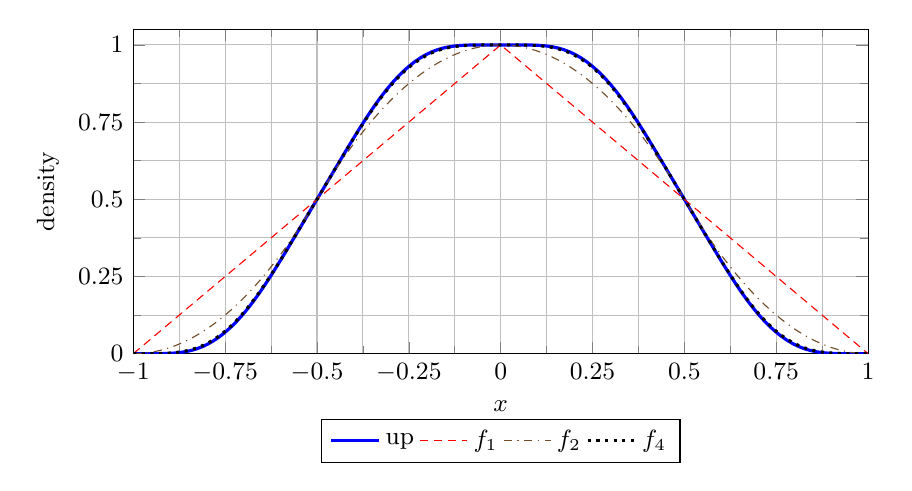
\begin{tikzpicture}
\begin{axis}[
  width=0.90\textwidth,
  height=0.47\textwidth,
  xmin=-1,xmax=1,ymin=0,ymax=1.05,
  xlabel={$x$},ylabel={density},
  xtick={-1,-0.75,-0.5,-0.25,0,0.25,0.5,0.75,1},
  ytick={0,0.25,0.5,0.75,1},
  grid=both,
  minor tick num=1,
  tick label style={font=\small},
  label style={font=\small},
  legend style={font=\small,at={(0.5,-0.20)},anchor=north,legend columns=4},
]
\addplot+[mark=none,line width=1.15pt] coordinates {
(-1.00000000,0.0000000000)
(-0.98437500,0.0000000021)
(-0.96875000,0.0000005727)
(-0.95312500,0.0000104681)
(-0.93750000,0.0000689621)
(-0.92187500,0.0002681716)
(-0.90625000,0.0007601198)
(-0.89062500,0.0017496732)
(-0.87500000,0.0034722156)
(-0.85937500,0.0061713187)
(-0.84375000,0.0100905539)
(-0.82812500,0.0154653054)
(-0.81250000,0.0225004393)
(-0.79687500,0.0313479791)
(-0.78125000,0.0421000415)
(-0.76562500,0.0547959004)
(-0.75000000,0.0694443120)
(-0.73437500,0.0860458408)
(-0.71875000,0.1045999223)
(-0.70312500,0.1250978002)
(-0.68750000,0.1475002009)
(-0.67187500,0.1717150073)
(-0.65625000,0.1975901963)
(-0.64062500,0.2249209014)
(-0.62500000,0.2534717388)
(-0.60937500,0.2829991368)
(-0.59375000,0.3132595238)
(-0.57812500,0.3440175159)
(-0.56250000,0.3750682468)
(-0.54687500,0.4062596932)
(-0.53125000,0.4374997382)
(-0.51562500,0.4687491080)
(-0.50000000,0.4999990463)
(-0.48437500,0.5312489847)
(-0.46875000,0.5624983544)
(-0.45312500,0.5937383994)
(-0.43750000,0.6249298458)
(-0.42187500,0.6559805767)
(-0.40625000,0.6867385689)
(-0.39062500,0.7169989559)
(-0.37500000,0.7465263539)
(-0.35937500,0.7750771912)
(-0.34375000,0.8024078964)
(-0.32812500,0.8282830853)
(-0.31250000,0.8524978917)
(-0.29687500,0.8749002924)
(-0.28125000,0.8953981704)
(-0.26562500,0.9139522519)
(-0.25000000,0.9305537806)
(-0.23437500,0.9452021923)
(-0.21875000,0.9578980512)
(-0.20312500,0.9686501136)
(-0.18750000,0.9774976533)
(-0.17187500,0.9845327873)
(-0.15625000,0.9899075387)
(-0.14062500,0.9938267740)
(-0.12500000,0.9965258770)
(-0.10937500,0.9982484195)
(-0.09375000,0.9992379728)
(-0.07812500,0.9997299211)
(-0.06250000,0.9999291306)
(-0.04687500,0.9999876246)
(-0.03125000,0.9999975200)
(-0.01562500,0.9999980906)
(0.00000000,0.9999980927)
(0.01562500,0.9999980906)
(0.03125000,0.9999975200)
(0.04687500,0.9999876246)
(0.06250000,0.9999291306)
(0.07812500,0.9997299211)
(0.09375000,0.9992379728)
(0.10937500,0.9982484195)
(0.12500000,0.9965258770)
(0.14062500,0.9938267740)
(0.15625000,0.9899075387)
(0.17187500,0.9845327873)
(0.18750000,0.9774976533)
(0.20312500,0.9686501136)
(0.21875000,0.9578980512)
(0.23437500,0.9452021923)
(0.25000000,0.9305537806)
(0.26562500,0.9139522519)
(0.28125000,0.8953981704)
(0.29687500,0.8749002924)
(0.31250000,0.8524978917)
(0.32812500,0.8282830853)
(0.34375000,0.8024078964)
(0.35937500,0.7750771912)
(0.37500000,0.7465263539)
(0.39062500,0.7169989559)
(0.40625000,0.6867385689)
(0.42187500,0.6559805767)
(0.43750000,0.6249298458)
(0.45312500,0.5937383994)
(0.46875000,0.5624983544)
(0.48437500,0.5312489847)
(0.50000000,0.4999990463)
(0.51562500,0.4687491080)
(0.53125000,0.4374997382)
(0.54687500,0.4062596932)
(0.56250000,0.3750682468)
(0.57812500,0.3440175159)
(0.59375000,0.3132595238)
(0.60937500,0.2829991368)
(0.62500000,0.2534717388)
(0.64062500,0.2249209014)
(0.65625000,0.1975901963)
(0.67187500,0.1717150073)
(0.68750000,0.1475002009)
(0.70312500,0.1250978002)
(0.71875000,0.1045999223)
(0.73437500,0.0860458408)
(0.75000000,0.0694443120)
(0.76562500,0.0547959004)
(0.78125000,0.0421000415)
(0.79687500,0.0313479791)
(0.81250000,0.0225004393)
(0.82812500,0.0154653054)
(0.84375000,0.0100905539)
(0.85937500,0.0061713187)
(0.87500000,0.0034722156)
(0.89062500,0.0017496732)
(0.90625000,0.0007601198)
(0.92187500,0.0002681716)
(0.93750000,0.0000689621)
(0.95312500,0.0000104681)
(0.96875000,0.0000005727)
(0.98437500,0.0000000021)
(1.00000000,0.0000000000)
};
\addlegendentry{$\Up$}
\addplot+[mark=none,densely dashed] coordinates {
(-1.00000000,0.0000000000)
(-0.98437500,0.0156240463)
(-0.96875000,0.0312490463)
(-0.95312500,0.0468740463)
(-0.93750000,0.0624990463)
(-0.92187500,0.0781240463)
(-0.90625000,0.0937490463)
(-0.89062500,0.1093740463)
(-0.87500000,0.1249990463)
(-0.85937500,0.1406240463)
(-0.84375000,0.1562490463)
(-0.82812500,0.1718740463)
(-0.81250000,0.1874990463)
(-0.79687500,0.2031240463)
(-0.78125000,0.2187490463)
(-0.76562500,0.2343740463)
(-0.75000000,0.2499990463)
(-0.73437500,0.2656240463)
(-0.71875000,0.2812490463)
(-0.70312500,0.2968740463)
(-0.68750000,0.3124990463)
(-0.67187500,0.3281240463)
(-0.65625000,0.3437490463)
(-0.64062500,0.3593740463)
(-0.62500000,0.3749990463)
(-0.60937500,0.3906240463)
(-0.59375000,0.4062490463)
(-0.57812500,0.4218740463)
(-0.56250000,0.4374990463)
(-0.54687500,0.4531240463)
(-0.53125000,0.4687490463)
(-0.51562500,0.4843740463)
(-0.50000000,0.4999990463)
(-0.48437500,0.5156240463)
(-0.46875000,0.5312490463)
(-0.45312500,0.5468740463)
(-0.43750000,0.5624990463)
(-0.42187500,0.5781240463)
(-0.40625000,0.5937490463)
(-0.39062500,0.6093740463)
(-0.37500000,0.6249990463)
(-0.35937500,0.6406240463)
(-0.34375000,0.6562490463)
(-0.32812500,0.6718740463)
(-0.31250000,0.6874990463)
(-0.29687500,0.7031240463)
(-0.28125000,0.7187490463)
(-0.26562500,0.7343740463)
(-0.25000000,0.7499990463)
(-0.23437500,0.7656240463)
(-0.21875000,0.7812490463)
(-0.20312500,0.7968740463)
(-0.18750000,0.8124990463)
(-0.17187500,0.8281240463)
(-0.15625000,0.8437490463)
(-0.14062500,0.8593740463)
(-0.12500000,0.8749990463)
(-0.10937500,0.8906240463)
(-0.09375000,0.9062490463)
(-0.07812500,0.9218740463)
(-0.06250000,0.9374990463)
(-0.04687500,0.9531240463)
(-0.03125000,0.9687490463)
(-0.01562500,0.9843740463)
(0.00000000,0.9999980927)
(0.01562500,0.9843740463)
(0.03125000,0.9687490463)
(0.04687500,0.9531240463)
(0.06250000,0.9374990463)
(0.07812500,0.9218740463)
(0.09375000,0.9062490463)
(0.10937500,0.8906240463)
(0.12500000,0.8749990463)
(0.14062500,0.8593740463)
(0.15625000,0.8437490463)
(0.17187500,0.8281240463)
(0.18750000,0.8124990463)
(0.20312500,0.7968740463)
(0.21875000,0.7812490463)
(0.23437500,0.7656240463)
(0.25000000,0.7499990463)
(0.26562500,0.7343740463)
(0.28125000,0.7187490463)
(0.29687500,0.7031240463)
(0.31250000,0.6874990463)
(0.32812500,0.6718740463)
(0.34375000,0.6562490463)
(0.35937500,0.6406240463)
(0.37500000,0.6249990463)
(0.39062500,0.6093740463)
(0.40625000,0.5937490463)
(0.42187500,0.5781240463)
(0.43750000,0.5624990463)
(0.45312500,0.5468740463)
(0.46875000,0.5312490463)
(0.48437500,0.5156240463)
(0.50000000,0.4999990463)
(0.51562500,0.4843740463)
(0.53125000,0.4687490463)
(0.54687500,0.4531240463)
(0.56250000,0.4374990463)
(0.57812500,0.4218740463)
(0.59375000,0.4062490463)
(0.60937500,0.3906240463)
(0.62500000,0.3749990463)
(0.64062500,0.3593740463)
(0.65625000,0.3437490463)
(0.67187500,0.3281240463)
(0.68750000,0.3124990463)
(0.70312500,0.2968740463)
(0.71875000,0.2812490463)
(0.73437500,0.2656240463)
(0.75000000,0.2499990463)
(0.76562500,0.2343740463)
(0.78125000,0.2187490463)
(0.79687500,0.2031240463)
(0.81250000,0.1874990463)
(0.82812500,0.1718740463)
(0.84375000,0.1562490463)
(0.85937500,0.1406240463)
(0.87500000,0.1249990463)
(0.89062500,0.1093740463)
(0.90625000,0.0937490463)
(0.92187500,0.0781240463)
(0.93750000,0.0624990463)
(0.95312500,0.0468740463)
(0.96875000,0.0312490463)
(0.98437500,0.0156240463)
(1.00000000,0.0000000000)
};
\addlegendentry{$f_1$}
\addplot+[mark=none,dashdotted] coordinates {
(-1.00000000,0.0000000000)
(-0.98437500,0.0004882515)
(-0.96875000,0.0019530654)
(-0.95312500,0.0043944418)
(-0.93750000,0.0078123808)
(-0.92187500,0.0122068822)
(-0.90625000,0.0175779462)
(-0.89062500,0.0239255726)
(-0.87500000,0.0312497616)
(-0.85937500,0.0395505130)
(-0.84375000,0.0488278270)
(-0.82812500,0.0590817034)
(-0.81250000,0.0703121424)
(-0.79687500,0.0825191438)
(-0.78125000,0.0957027078)
(-0.76562500,0.1098628342)
(-0.75000000,0.1249995232)
(-0.73437500,0.1411127746)
(-0.71875000,0.1582025886)
(-0.70312500,0.1762689650)
(-0.68750000,0.1953119040)
(-0.67187500,0.2153314054)
(-0.65625000,0.2363274694)
(-0.64062500,0.2583000958)
(-0.62500000,0.2812492847)
(-0.60937500,0.3051750362)
(-0.59375000,0.3300773501)
(-0.57812500,0.3559562266)
(-0.56250000,0.3828116655)
(-0.54687500,0.4106436670)
(-0.53125000,0.4394522309)
(-0.51562500,0.4692373574)
(-0.50000000,0.4999990463)
(-0.48437500,0.5307607353)
(-0.46875000,0.5605458617)
(-0.45312500,0.5893544257)
(-0.43750000,0.6171864271)
(-0.42187500,0.6440418661)
(-0.40625000,0.6699207425)
(-0.39062500,0.6948230565)
(-0.37500000,0.7187488079)
(-0.35937500,0.7416979969)
(-0.34375000,0.7636706233)
(-0.32812500,0.7846666872)
(-0.31250000,0.8046861887)
(-0.29687500,0.8237291276)
(-0.28125000,0.8417955041)
(-0.26562500,0.8588853180)
(-0.25000000,0.8749985695)
(-0.23437500,0.8901352584)
(-0.21875000,0.9042953849)
(-0.20312500,0.9174789488)
(-0.18750000,0.9296859503)
(-0.17187500,0.9409163892)
(-0.15625000,0.9511702657)
(-0.14062500,0.9604475796)
(-0.12500000,0.9687483311)
(-0.10937500,0.9760725200)
(-0.09375000,0.9824201465)
(-0.07812500,0.9877912104)
(-0.06250000,0.9921857119)
(-0.04687500,0.9956036508)
(-0.03125000,0.9980450273)
(-0.01562500,0.9995098412)
(0.00000000,0.9999980927)
(0.01562500,0.9995098412)
(0.03125000,0.9980450273)
(0.04687500,0.9956036508)
(0.06250000,0.9921857119)
(0.07812500,0.9877912104)
(0.09375000,0.9824201465)
(0.10937500,0.9760725200)
(0.12500000,0.9687483311)
(0.14062500,0.9604475796)
(0.15625000,0.9511702657)
(0.17187500,0.9409163892)
(0.18750000,0.9296859503)
(0.20312500,0.9174789488)
(0.21875000,0.9042953849)
(0.23437500,0.8901352584)
(0.25000000,0.8749985695)
(0.26562500,0.8588853180)
(0.28125000,0.8417955041)
(0.29687500,0.8237291276)
(0.31250000,0.8046861887)
(0.32812500,0.7846666872)
(0.34375000,0.7636706233)
(0.35937500,0.7416979969)
(0.37500000,0.7187488079)
(0.39062500,0.6948230565)
(0.40625000,0.6699207425)
(0.42187500,0.6440418661)
(0.43750000,0.6171864271)
(0.45312500,0.5893544257)
(0.46875000,0.5605458617)
(0.48437500,0.5307607353)
(0.50000000,0.4999990463)
(0.51562500,0.4692373574)
(0.53125000,0.4394522309)
(0.54687500,0.4106436670)
(0.56250000,0.3828116655)
(0.57812500,0.3559562266)
(0.59375000,0.3300773501)
(0.60937500,0.3051750362)
(0.62500000,0.2812492847)
(0.64062500,0.2583000958)
(0.65625000,0.2363274694)
(0.67187500,0.2153314054)
(0.68750000,0.1953119040)
(0.70312500,0.1762689650)
(0.71875000,0.1582025886)
(0.73437500,0.1411127746)
(0.75000000,0.1249995232)
(0.76562500,0.1098628342)
(0.78125000,0.0957027078)
(0.79687500,0.0825191438)
(0.81250000,0.0703121424)
(0.82812500,0.0590817034)
(0.84375000,0.0488278270)
(0.85937500,0.0395505130)
(0.87500000,0.0312497616)
(0.89062500,0.0239255726)
(0.90625000,0.0175779462)
(0.92187500,0.0122068822)
(0.93750000,0.0078123808)
(0.95312500,0.0043944418)
(0.96875000,0.0019530654)
(0.98437500,0.0004882515)
(1.00000000,0.0000000000)
};
\addlegendentry{$f_2$}
\addplot+[mark=none,dotted,line width=1.1pt] coordinates {
(-1.00000000,0.0000000000)
(-0.98437500,0.0000012715)
(-0.96875000,0.0000203447)
(-0.95312500,0.0001029958)
(-0.93750000,0.0003255184)
(-0.92187500,0.0007947237)
(-0.90625000,0.0016479408)
(-0.89062500,0.0030530161)
(-0.87500000,0.0052083135)
(-0.85937500,0.0083401715)
(-0.84375000,0.0126749287)
(-0.82812500,0.0184109489)
(-0.81250000,0.0257160788)
(-0.79687500,0.0347276471)
(-0.78125000,0.0455524651)
(-0.76562500,0.0582668266)
(-0.75000000,0.0729165077)
(-0.73437500,0.0895167670)
(-0.71875000,0.1080523459)
(-0.70312500,0.1284774683)
(-0.68750000,0.1507158404)
(-0.67187500,0.1746606509)
(-0.65625000,0.2001745710)
(-0.64062500,0.2270897543)
(-0.62500000,0.2552078366)
(-0.60937500,0.2843024796)
(-0.59375000,0.3141473448)
(-0.57812500,0.3445440681)
(-0.56250000,0.3753248031)
(-0.54687500,0.4063522209)
(-0.53125000,0.4375195103)
(-0.51562500,0.4687503775)
(-0.50000000,0.4999990463)
(-0.48437500,0.5312477152)
(-0.46875000,0.5624785824)
(-0.45312500,0.5936458717)
(-0.43750000,0.6246732896)
(-0.42187500,0.6554540246)
(-0.40625000,0.6858507479)
(-0.39062500,0.7156956130)
(-0.37500000,0.7447902560)
(-0.35937500,0.7729083384)
(-0.34375000,0.7998235216)
(-0.32812500,0.8253374417)
(-0.31250000,0.8492822523)
(-0.29687500,0.8715206244)
(-0.28125000,0.8919457467)
(-0.26562500,0.9104813256)
(-0.25000000,0.9270815849)
(-0.23437500,0.9417312660)
(-0.21875000,0.9544456275)
(-0.20312500,0.9652704456)
(-0.18750000,0.9742820139)
(-0.17187500,0.9815871437)
(-0.15625000,0.9873231640)
(-0.14062500,0.9916579211)
(-0.12500000,0.9947897792)
(-0.10937500,0.9969450766)
(-0.09375000,0.9983501518)
(-0.07812500,0.9992033689)
(-0.06250000,0.9996725743)
(-0.04687500,0.9998950969)
(-0.03125000,0.9999777479)
(-0.01562500,0.9999968211)
(0.00000000,0.9999980927)
(0.01562500,0.9999968211)
(0.03125000,0.9999777479)
(0.04687500,0.9998950969)
(0.06250000,0.9996725743)
(0.07812500,0.9992033689)
(0.09375000,0.9983501518)
(0.10937500,0.9969450766)
(0.12500000,0.9947897792)
(0.14062500,0.9916579211)
(0.15625000,0.9873231640)
(0.17187500,0.9815871437)
(0.18750000,0.9742820139)
(0.20312500,0.9652704456)
(0.21875000,0.9544456275)
(0.23437500,0.9417312660)
(0.25000000,0.9270815849)
(0.26562500,0.9104813256)
(0.28125000,0.8919457467)
(0.29687500,0.8715206244)
(0.31250000,0.8492822523)
(0.32812500,0.8253374417)
(0.34375000,0.7998235216)
(0.35937500,0.7729083384)
(0.37500000,0.7447902560)
(0.39062500,0.7156956130)
(0.40625000,0.6858507479)
(0.42187500,0.6554540246)
(0.43750000,0.6246732896)
(0.45312500,0.5936458717)
(0.46875000,0.5624785824)
(0.48437500,0.5312477152)
(0.50000000,0.4999990463)
(0.51562500,0.4687503775)
(0.53125000,0.4375195103)
(0.54687500,0.4063522209)
(0.56250000,0.3753248031)
(0.57812500,0.3445440681)
(0.59375000,0.3141473448)
(0.60937500,0.2843024796)
(0.62500000,0.2552078366)
(0.64062500,0.2270897543)
(0.65625000,0.2001745710)
(0.67187500,0.1746606509)
(0.68750000,0.1507158404)
(0.70312500,0.1284774683)
(0.71875000,0.1080523459)
(0.73437500,0.0895167670)
(0.75000000,0.0729165077)
(0.76562500,0.0582668266)
(0.78125000,0.0455524651)
(0.79687500,0.0347276471)
(0.81250000,0.0257160788)
(0.82812500,0.0184109489)
(0.84375000,0.0126749287)
(0.85937500,0.0083401715)
(0.87500000,0.0052083135)
(0.89062500,0.0030530161)
(0.90625000,0.0016479408)
(0.92187500,0.0007947237)
(0.93750000,0.0003255184)
(0.95312500,0.0001029958)
(0.96875000,0.0000203447)
(0.98437500,0.0000012715)
(1.00000000,0.0000000000)
};
\addlegendentry{$f_4$}
\end{axis}
\end{tikzpicture}
\caption{The first smooth finite box splines and their limit.  The plotted up-function is a
high-stage numerical evaluation used only for illustration.}
\label{fig:iterates}
\end{figure}

\section{Fourier product and exact identification of the limit}
\label{sec:fourier}

Under the Fourier convention fixed above,
\begin{equation}
 \widehat{\beta_a}(\xi)=\sinc(a\xi).                       \label{eq:box-fourier}
\end{equation}
Therefore \Cref{thm:box-convolution} gives the transform conjectured in the original question,
without any induction through piecewise polynomials.

\begin{theorem}[Finite Fourier product]
\label{thm:finite-fourier}
For every $n\ge1$,
\begin{align}
 \widehat f_n(\xi)
 &=\sinc(2^{-n}\xi)\prod_{k=1}^{n}\sinc(2^{-k}\xi)         \label{eq:fn-fourier}\\
 &=\left(\prod_{k=1}^{n-1}\sinc(2^{-k}\xi)\right)
   \sinc^2(2^{-n}\xi).                                     \label{eq:fn-fourier-duplicate}
\end{align}
As $n\to\infty$, this converges pointwise to \eqref{eq:up-fourier}.
\end{theorem}

The extra front factor in the Stack Exchange formula is now transparent: it is the Fourier
transform of the duplicated smallest box.  It is not an arbitrary normalization correction;
it records the support-filling tail replacement.

A useful formula for the operator itself is
\begin{equation}
 \widehat{Tg}(\xi)=\sinc(\xi/2)\widehat g(\xi/2).           \label{eq:T-fourier}
\end{equation}
Iterating \eqref{eq:T-fourier} from $\widehat\rho(\xi)=\sinc\xi$ gives
\eqref{eq:fn-fourier} directly.  Passing to the limit gives the unique continuous transform
with value $1$ at the origin that solves the fixed-point equation.

\begin{corollary}[Strong convergence in every fixed smoothness order]
\label{cor:Cm-convergence}
For every fixed $m\ge0$,
\begin{equation}
 \max_{0\le r\le m}\norm{f_n^{(r)}-\Up^{(r)}}_\infty\longrightarrow0,        \label{eq:Cm-convergence}
\end{equation}
where $n$ is taken large enough that the indicated finite-stage derivatives exist.
\end{corollary}

\begin{proof}
Fix $M>m+2$.  For $n\ge M$, the first $M$ sinc factors in \eqref{eq:fn-fourier} supply an
integrable majorant after multiplication by $|\xi|^m$, while every remaining sinc factor has
modulus at most one.  Dominated convergence and Fourier inversion give uniform convergence of
each derivative through order $m$.  A much sharper and exact estimate is proved in
\Cref{sec:exact-rate}.
\end{proof}

\section{The exact \texorpdfstring{$n$th}{n-th} stage in truncated powers}
\label{sec:closed-form}

The positive-part notation is
\[
 \pos y^r=\begin{cases}y^r,&y>0,\\0,&y\le0.\end{cases}
\]
For $r>0$ the value at $y=0$ is immaterial.  The following standard box-spline identity is the
closed form behind the repeated integrations.

\begin{lemma}[A convolution of arbitrary boxes]
\label{lem:general-box-spline}
Let $a_1,\ldots,a_N>0$, put $A=\sum_{i=1}^{N}a_i$, and let
$\beta_{a_i}$ be as in \eqref{eq:beta}.  Then
\begin{equation}
 (\beta_{a_1}*\cdots*\beta_{a_N})(x)
 =\frac{1}{(N-1)!\prod_{i=1}^{N}(2a_i)}
 \sum_{S\subseteq\{1,\ldots,N\}}(-1)^{|S|}
 \pos{x+A-2\sum_{i\in S}a_i}^{N-1}.                       \label{eq:general-box-spline}
\end{equation}
\end{lemma}

\begin{proof}
Write
$\beta_a=(2a)^{-1}(H(\,\boldsymbol\cdot+a)-H(\,\boldsymbol\cdot-a))$, where $H$ is the
Heaviside distribution.  Expanding the $N$ binary differences gives one term for every
subset $S$.  The $N$-fold convolution of Heaviside functions is
$\pos x^{N-1}/(N-1)!$.  Translating by the sum of the selected endpoints gives
\eqref{eq:general-box-spline}.  The same proof can be written as an induction by integrating
one more moving interval at each step.
\end{proof}

For the dyadic widths in \eqref{eq:fn-box}, the total half-width is $A=1$ and
\begin{equation}
 \left(\prod_{k=1}^{n}2\cdot2^{-k}\right)(2\cdot2^{-n})
 =2^{1-\binom{n+1}{2}}.                                    \label{eq:normalization-product}
\end{equation}
This gives a direct subset formula.

\begin{theorem}[Exact subset-sum formula]
\label{thm:subset-formula}
For $n\ge1$, let
\[
 a_1=2^{-1},\ldots,a_n=2^{-n},\qquad a_{n+1}=2^{-n}.
\]
Then
\begin{equation}
 f_n(x)=\frac{2^{\binom{n+1}{2}-1}}{n!}
 \sum_{S\subseteq\{1,\ldots,n+1\}}(-1)^{|S|}
 \pos{x+1-2\sum_{i\in S}a_i}^{n}.                         \label{eq:subset-formula}
\end{equation}
\end{theorem}

The binary subset sums of the first $n$ distinct boxes are unique.  This is where the
Thue--Morse signs enter.

\begin{definition}[Finite Thue--Morse row]
For a fixed $n\ge1$, define
\begin{equation}
 c_n(j)=
 \begin{cases}
  (-1)^{\wt(j)},&0\le j<2^n,\\
  0,&\text{otherwise}.
 \end{cases}                                                \label{eq:cn}
\end{equation}
Write $\Delta c_n(j)=c_n(j)-c_n(j-1)$.
\end{definition}

\begin{theorem}[Exact Thue--Morse closed form]
\label{thm:TM-formula}
For every $n\ge1$ and $x\in\R$,
\begin{equation}
 \boxed{\displaystyle
 f_n(x)=\frac{2^{\binom{n+1}{2}-1}}{n!}
 \sum_{j=0}^{2^n}\Delta c_n(j)
 \pos{x+1-\frac{j}{2^{n-1}}}^{n}.}                         \label{eq:TM-formula}
\end{equation}
Equivalently, away from the dyadic breakpoints, the sum may be stopped at
$j=\lfloor2^{n-1}(x+1)\rfloor$.
\end{theorem}

\begin{proof}
For a subset of the first $n$ boxes, the quantity
$2\sum a_i$ equals $j/2^{n-1}$, where the binary digits of $j$ record the chosen indices and
the sign is $(-1)^{\wt(j)}=c_n(j)$.  If the duplicated last box is not chosen, the coefficient
at $j$ is $c_n(j)$.  If it is chosen, its extra binary unit shifts $j-1$ to $j$ and reverses
the sign, contributing $-c_n(j-1)$.  Their sum is $\Delta c_n(j)$.  Substitute into
\eqref{eq:subset-formula}.
\end{proof}

Formula \eqref{eq:TM-formula} is algebraically equivalent to the 2012 answer
\cite{mseanswer}.  The present derivation shows why the coefficient is a \emph{difference} of
two consecutive Thue--Morse signs: it is exactly the collision caused by the duplicated
smallest box.

\subsection{Knots, cells, and the highest derivative}

All possible breakpoints lie on the grid
\begin{equation}
 x_j=-1+\frac{j}{2^{n-1}},\qquad 0\le j\le2^n.             \label{eq:knot-grid}
\end{equation}
Some grid points are inactive because $\Delta c_n(j)$ can vanish.  Differentiating
\eqref{eq:TM-formula} $r$ times for $0\le r\le n-1$ gives
\begin{equation}
 f_n^{(r)}(x)=
 \frac{2^{\binom{n+1}{2}-1}}{(n-r)!}
 \sum_{j=0}^{2^n}\Delta c_n(j)
 \pos{x+1-\frac{j}{2^{n-1}}}^{n-r}.                        \label{eq:TM-derivatives}
\end{equation}
The $n$th derivative is a step function away from the grid.

\begin{corollary}[The $n$th derivative is a Thue--Morse step function]
\label{cor:nth-derivative}
If $-1<x<1$ and $x$ is not on the grid \eqref{eq:knot-grid}, put
\begin{equation}
 J=\left\lfloor2^{n-1}(x+1)\right\rfloor.
\end{equation}
Then
\begin{equation}
 f_n^{(n)}(x)=2^{\binom{n+1}{2}-1}(-1)^{\wt(J)}.            \label{eq:nth-derivative}
\end{equation}
\end{corollary}

\begin{proof}
After $n$ derivatives, each positive-part power becomes a Heaviside step.  On the indicated
cell, the active coefficients telescope:
\[
 \sum_{j=0}^{J}\Delta c_n(j)=c_n(J)=(-1)^{\wt(J)}.
\]
\end{proof}

This identity explains the derivative plots in the original question exactly: the finest
derivative is a rescaled Thue--Morse row, and every lower derivative is its successive
piecewise-polynomial integral.

\section{Tail replacement rather than truncation}
\label{sec:tail-replacement}

The random series makes the approximation mechanism exact.  Recall the prefix
\begin{equation}
 S_n=\sum_{k=1}^{n}2^{-k}U_k,
 \qquad \text{density }p_n.                                \label{eq:Sn}
\end{equation}
Split the infinite series at level $n$:
\begin{equation}
 Y=S_n+2^{-n}Y',                                           \label{eq:Y-tail}
\end{equation}
where $Y'$ is an independent copy of $Y$.  On the other hand,
\begin{equation}
 X_n=S_n+2^{-n}V,                                          \label{eq:X-tail}
\end{equation}
where $V\sim\Unif[-1,1]$ is independent.  Thus the finite iteration keeps the first $n$
dyadic boxes exactly and replaces the true self-similar tail by a uniform law on the same
support.

The two tail laws agree in their zeroth and first moments.  Their second moments are
\begin{equation}
 \E V^2=\frac13,
 \qquad
 \E Y^2=\frac13\sum_{k=1}^{\infty}4^{-k}=\frac19.          \label{eq:tail-variances}
\end{equation}
Consequently
\begin{equation}
 \Var(X_n)-\Var(Y)=\frac29\,4^{-n}.                        \label{eq:variance-defect}
\end{equation}
This already predicts a second-order error with coefficient $1/9$: a centered smoothing
error acts to first order like one half of the variance defect times a second derivative.
The next section turns this heuristic into an exact norm identity.

\section{A positive Peano kernel}
\label{sec:Peano}

Let
\begin{equation}
 h=\rho-\Up.                                                \label{eq:h}
\end{equation}
It is an even compactly supported signed density with zero total mass and zero first moment.
Define its twice-integrated kernel by
\begin{equation}
 K(x)=\frac12\int_{\R}|x-t|h(t)\dd t.                      \label{eq:K-def}
\end{equation}
Then $K''=h$ in the sense of distributions.  The essential fact is that $K$ is nonnegative.

\begin{proposition}[The tail Peano kernel]
\label{prop:K-properties}
The function $K$ has the following properties:
\begin{enumerate}
\item $K$ is even, belongs to $C^1(\R)$, is supported on $[-1,1]$, and satisfies $K''=\rho-\Up$;
\item $K(x)\ge0$ for all $x$, and $K$ is nonincreasing on $[0,1]$;
\item
\begin{equation}
 \int_{\R}K(x)\dd x=\frac19;                              \label{eq:K-mass}
\end{equation}
\item
\begin{equation}
 K(0)=\frac19.                                             \label{eq:K-zero}
\end{equation}
\end{enumerate}
\end{proposition}

\begin{proof}
Evenness and $C^1$ regularity follow directly from \eqref{eq:K-def}; two distributional
derivatives of $|x-t|/2$ give $\delta_t$.  For $x>1$, one has $|x-t|=x-t$ on the support of
$h$, so $K(x)=\tfrac12(x\int h-\int th)=0$.  The same argument applies for $x<-1$.

For $0\le x\le1$, differentiation gives the difference of the two cumulative distribution
functions:
\begin{equation}
 K'(x)=\frac{x}{2}-\int_0^x\Up(t)\dd t.                    \label{eq:K-prime}
\end{equation}
For $0<x<1$, the differential equation \eqref{eq:up-diffeq} and the support of $\Up$ give
$\Up'(x)=-2\Up(2x-1)\le0$.  Thus the up-function is nonincreasing on $[0,1]$; it
has integral $1/2$ there by evenness and normalization.  Hence the average of $\Up$ over
$[0,x]$ is at least its average over $[0,1]$, so
$\int_0^x\Up(t)\dd t\ge x/2$.  Thus $K'(x)\le0$.  Since $K(1)=0$, this proves $K\ge0$ on
$[0,1]$, and evenness handles the other half.

Integrating $K''=h$ twice by parts against $x^2$ and using the compact support of $K$ gives
\[
 2\int K(x)\dd x=\int x^2h(x)\dd x
 =\E V^2-\E Y^2=\frac13-\frac19=\frac29,
\]
which proves \eqref{eq:K-mass}.

Finally,
\[
 K(0)=\frac12\bigl(\E|V|-\E|Y|\bigr).
\]
Clearly $\E|V|=1/2$.  From the stationary identity
$Y\overset d=(U+Y')/2$, with $U$ uniform and $Y'$ an independent copy, and the elementary
formula
\[
 \E_U|U+y|=\frac12\int_{-1}^{1}|u+y|\dd u=\frac{1+y^2}{2}
 \qquad(|y|\le1),
\]
we obtain
\[
 \E|Y|=\frac14\bigl(1+\E Y^2\bigr)=\frac14\left(1+\frac19\right)=\frac5{18}.
\]
Therefore $K(0)=\tfrac12(\tfrac12-\tfrac5{18})=1/9$.
\end{proof}

\begin{remark}[Convex order]
The nonnegativity of $K$ is equivalent to
\begin{equation}
 Y\preceq_{\mathrm{cx}}V,                                  \label{eq:convex-order}
\end{equation}
meaning $\E\phi(Y)\le\E\phi(V)$ for every convex $\phi$ for which the expectations exist.
After adding the independent prefix and scaling, this gives
$Y\preceq_{\mathrm{cx}}X_n$.  The iterates are therefore systematically more dispersed than
the limiting law, even though they share the same support and mean.
\end{remark}

Scale the signed tail and its Peano kernel by
\begin{equation}
 h_n(t)=2^nh(2^nt),
 \qquad
 K_n(t)=2^{-n}K(2^nt).                                     \label{eq:scaled-K}
\end{equation}
Then
\begin{equation}
 K_n''=h_n,
 \qquad
 \supp K_n\subseteq[-2^{-n},2^{-n}],
 \qquad
 K_n\ge0,
 \qquad
 \int K_n=\frac{4^{-n}}9.                                 \label{eq:scaled-K-properties}
\end{equation}
The two exact tail factorizations \eqref{eq:Y-tail}--\eqref{eq:X-tail} now give
\begin{equation}
 f_n-\Up=p_n*h_n=p_n*K_n''=p_n''*K_n                       \label{eq:error-factorization}
\end{equation}
in the sense of distributions, and as an ordinary convolution whenever the displayed
derivatives are functions.  This is the central error identity.

\begin{corollary}[A sharp weak error bound]
\label{cor:weak-error}
For every $\phi\in C^2(\R)$ with bounded second derivative,
\begin{equation}
 \left|\E\phi(X_n)-\E\phi(Y)\right|
 \le\frac{4^{-n}}9\norm{\phi''}_\infty.                   \label{eq:weak-error}
\end{equation}
If $\phi$ is convex, the difference on the left before taking absolute values is nonnegative.
The constant is sharp, as seen from $\phi(x)=x^2$.
\end{corollary}

\begin{proof}
Pair \eqref{eq:error-factorization} with $\phi$, move the two derivatives onto $\phi$, and use
that $p_n$ is a probability density and $K_n$ is nonnegative of mass $4^{-n}/9$.
For $\phi(x)=x^2$, equality is exactly the variance defect \eqref{eq:variance-defect}.
\end{proof}

\section{A finite-prefix derivative plateau}
\label{sec:prefix-derivatives}

To turn \eqref{eq:error-factorization} into a sharp uniform estimate, one needs an exact bound
for derivatives of the prefix spline $p_n$.  The relevant constant is the same triangular
power of two that occurs in the sharp derivative bounds for $\Up$.

\begin{lemma}[Summatory Thue--Morse cancellation]
\label{lem:TM-prefix}
Let $\eps_j=(-1)^{\wt(j)}$.  Then for every $J\ge0$,
\begin{equation}
 \sum_{j=0}^{J}\eps_j=
 \begin{cases}
  \eps_{J/2},&J\text{ even},\\
  0,&J\text{ odd}.
 \end{cases}                                                \label{eq:TM-prefix}
\end{equation}
In particular, every prefix sum has absolute value at most one.
\end{lemma}

\begin{proof}
The identities $\eps_{2q}=\eps_q$ and $\eps_{2q+1}=-\eps_q$ make every complete adjacent pair
cancel.  An even endpoint leaves the last even term unpaired.
\end{proof}

\begin{theorem}[Exact derivative norm and a saturated interval]
\label{thm:prefix-plateau}
Let $r\ge0$ and $n\ge r+1$.  Put
\begin{equation}
 C_r=2^{\binom{r+1}{2}},
 \qquad
 x_r=-1+2^{-r}.                                             \label{eq:Cr-xr}
\end{equation}
Then the $r$th derivative of $p_n$ exists as a bounded piecewise function and satisfies
\begin{equation}
 \norm{p_n^{(r)}}_\infty=C_r.                              \label{eq:pn-derivative-norm}
\end{equation}
More precisely,
\begin{equation}
 p_n^{(r)}(x)=C_r
 \quad\text{for almost every }x\in[x_r-2^{-n},x_r+2^{-n}]. \label{eq:pn-plateau}
\end{equation}
\end{theorem}

\begin{proof}
First take $n=r+1$.  Applying \Cref{lem:general-box-spline} to the $r+1$ distinct boxes in
$p_{r+1}$ and differentiating $r$ times gives a step function.  Its possible knots are
\[
 -\left(1-2^{-(r+1)}\right)+\frac{j}{2^r},
 \qquad 0\le j<2^{r+1},
\]
and its value on the cell after the $J$th knot is
\[
 2^{\binom{r+1}{2}}\sum_{j=0}^{J}(-1)^{\wt(j)}.
\]
By \Cref{lem:TM-prefix}, its absolute value is at most $C_r$.  On the first cell the prefix
sum is $1$, so the value is $C_r$.  That first cell is centered at $x_r=-1+2^{-r}$ and has
half-width $2^{-(r+1)}$.

For larger $n$, factor
\[
 p_n=p_{r+1}*\beta_{2^{-(r+2)}}*\cdots*\beta_{2^{-n}}
     =p_{r+1}*q_{r,n},
\]
where $q_{r,n}$ is a probability density supported in the interval of radius
\[
 \sum_{k=r+2}^{n}2^{-k}=2^{-(r+1)}-2^{-n}.
\]
Therefore $p_n^{(r)}=p_{r+1}^{(r)}*q_{r,n}$ has norm at most $C_r$.  If
$|x-x_r|\le2^{-n}$, then every point $x-t$ sampled by the convolution remains in the first
cell of $p_{r+1}^{(r)}$, except possibly at its null endpoints.  Hence the convolution equals
$C_r$ there.  This proves both the upper bound and its attainment.
\end{proof}

\begin{remark}
The limiting sharp bound in the companion document is
$\norm{\Up^{(r)}}_\infty=C_r$, attained at the same dyadic point $x_r$ \cite{companion}.
\Cref{thm:prefix-plateau} explains this without taking a limit: every sufficiently long finite
prefix already has the exact extremal height, and the plateau shrinks to the extremal point.
\end{remark}

\section{The exact convergence rate}
\label{sec:exact-rate}

We now combine the positive kernel \eqref{eq:error-factorization} with the saturated derivative
interval \eqref{eq:pn-plateau}.

\begin{theorem}[Exact $C^m$ error]
\label{thm:exact-Cm-error}
Let $m\ge0$ and $n\ge m+3$.  Then
\begin{equation}
 \boxed{\displaystyle
 \norm{f_n^{(m)}-\Up^{(m)}}_\infty
 =\frac{2^{\binom{m+3}{2}}}{9}\,4^{-n}.}                  \label{eq:exact-Cm-error}
\end{equation}
The positive maximum is attained at
\begin{equation}
 x=-1+2^{-(m+2)}.                                          \label{eq:error-extremal-point}
\end{equation}
\end{theorem}

\begin{proof}
Differentiate \eqref{eq:error-factorization} $m$ times and put $r=m+2$:
\begin{equation}
 f_n^{(m)}-\Up^{(m)}=p_n^{(r)}*K_n.                        \label{eq:error-r}
\end{equation}
The kernel is nonnegative and has mass $4^{-n}/9$, while
$\norm{p_n^{(r)}}_\infty=C_r=2^{\binom{m+3}{2}}$ by
\Cref{thm:prefix-plateau}.  Therefore
\[
 \norm{f_n^{(m)}-\Up^{(m)}}_\infty
 \le C_r\int K_n
 =\frac{C_r}{9}4^{-n}.
\]
At $x=x_r=-1+2^{-r}$, the interval $x_r-\supp K_n$ is exactly contained in the saturated
interval \eqref{eq:pn-plateau}.  Hence the integrand in \eqref{eq:error-r} equals $C_r$ almost
everywhere on the support of $K_n$, and
\[
 (f_n^{(m)}-\Up^{(m)})(x_r)=C_r\int K_n=\frac{C_r}{9}4^{-n}.
\]
The upper bound is therefore an equality.
\end{proof}

For $m=0$, the theorem directly covers $n\ge3$.  The second stage has one derivative too few
for the preceding $L^\infty$ argument, but the distributional formula can be evaluated
explicitly.

\begin{proposition}[The exceptional second stage]
\label{prop:n2-error}
One has
\begin{equation}
 \norm{f_2-\Up}_\infty=\frac1{18}=\frac89\,4^{-2}.         \label{eq:n2-error}
\end{equation}
\end{proposition}

\begin{proof}
The prefix $p_2=\beta_{1/2}*\beta_{1/4}$ is a trapezoid, and its distributional second
derivative is
\begin{equation}
 p_2''=2\bigl(\delta_{-3/4}-\delta_{-1/4}-\delta_{1/4}+\delta_{3/4}\bigr).    \label{eq:p2-second}
\end{equation}
Thus \eqref{eq:error-factorization} gives
\begin{align}
 f_2(x)-\Up(x)=2\bigl(&K_2(x+3/4)-K_2(x+1/4)\notag\\
                     &-K_2(x-1/4)+K_2(x-3/4)\bigr).        \label{eq:e2-K}
\end{align}
The four translates have disjoint interiors because $K_2$ is supported on $[-1/4,1/4]$.
Since $K$ is even and decreases on $[0,1]$, its maximum is $K(0)=1/9$, so
$\max K_2=2^{-2}K(0)=1/36$.  Therefore the maximum absolute value in \eqref{eq:e2-K} is
$2/36=1/18$, attained at the four translation centers.
\end{proof}

The first two stages can also be evaluated exactly.  The initial error is plainly $1/2$.  For
$f_1$, use \eqref{eq:F-up}: on $0\le x\le1$,
\begin{equation}
 f_1(x)-\Up(x)=1-x-F(1-x)=F(x)-x.                          \label{eq:e1-F}
\end{equation}
On $[0,1/2]$ its derivative is $2F(2x)-1$, which changes sign only at $x=1/4$.  The already
established dyadic value $F(1/4)=5/72$ then gives the extremal value $-13/72$; symmetry about
$1/2$ gives $+13/72$ at $3/4$.

\begin{theorem}[Complete exact uniform-error sequence]
\label{thm:complete-error}
For every $n\ge0$,
\begin{equation}
 \boxed{\displaystyle
 \norm{f_n-\Up}_\infty=
 \begin{cases}
  \frac12,&n=0,\\[0.25em]
  \frac{13}{72},&n=1,\\[0.25em]
  \frac89\,4^{-n},&n\ge2.
 \end{cases}}                                              \label{eq:complete-error}
\end{equation}
For $n\ge2$,
\begin{equation}
 \begin{aligned}
 f_n(\pm3/4)-\Up(\pm3/4)&=+\frac89\,4^{-n},\\
 f_n(\pm1/4)-\Up(\pm1/4)&=-\frac89\,4^{-n}.
 \end{aligned}                                             \label{eq:four-extrema}
\end{equation}
\end{theorem}

\begin{proof}
The cases $n=0,1$ were just discussed, $n=2$ is \Cref{prop:n2-error}, and $n\ge3$ is
\Cref{thm:exact-Cm-error} with $m=0$.  The four signed extrema follow from the four plateaux
of height $\pm8$ in the second derivative of the three-box prefix, preserved by all later
probability convolutions; equivalently they follow directly from \eqref{eq:e2-K} and the same
plateau argument used in \Cref{thm:exact-Cm-error}.
\end{proof}

Since $\Up(3/4)=F(1/4)=5/72$ and $\Up(1/4)=F(3/4)=67/72$, the extremal values themselves are
\begin{equation}
 f_n(3/4)=\frac5{72}+\frac8{9\,4^n},
 \qquad
 f_n(1/4)=\frac{67}{72}-\frac8{9\,4^n}
 \qquad(n\ge2).                                            \label{eq:extremal-values}
\end{equation}
For example,
\begin{center}
\begin{tabular}{c@{\qquad}c@{\qquad}c}
\toprule
$n$ & $f_n(3/4)$ & $4^n\bigl(f_n(3/4)-\Up(3/4)\bigr)$\\
\midrule
2 & $1/8$ & $8/9$\\
3 & $1/12$ & $8/9$\\
4 & $7/96$ & $8/9$\\
5 & $9/128$ & $8/9$\\
6 & $107/1536$ & $8/9$\\
\bottomrule
\end{tabular}
\end{center}

\begin{figure}[htbp]
\centering
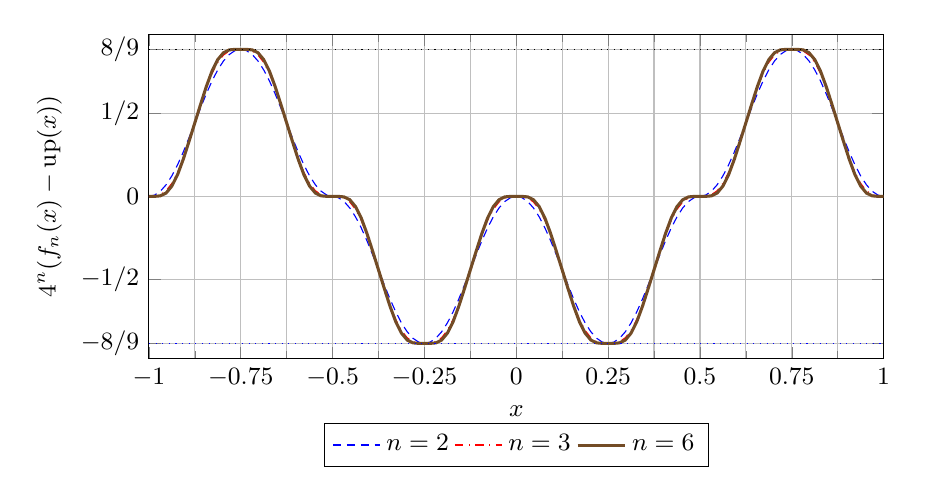
\begin{tikzpicture}
\begin{axis}[
  width=0.90\textwidth,
  height=0.47\textwidth,
  xmin=-1,xmax=1,ymin=-0.98,ymax=0.98,
  xlabel={$x$},ylabel={$4^n(f_n(x)-\Up(x))$},
  xtick={-1,-0.75,-0.5,-0.25,0,0.25,0.5,0.75,1},
  ytick={-0.8888889,-0.5,0,0.5,0.8888889},
  yticklabels={$-8/9$,$-1/2$,$0$,$1/2$,$8/9$},
  grid=both,
  minor tick num=1,
  tick label style={font=\small},
  label style={font=\small},
  legend style={font=\small,at={(0.5,-0.20)},anchor=north,legend columns=3},
]
\addplot+[mark=none,densely dashed] coordinates {
(-1.00000000,0.0000000000)
(-0.98437500,0.0078119904)
(-0.96875000,0.0312398836)
(-0.95312500,0.0701435800)
(-0.93750000,0.1238946997)
(-0.92187500,0.1910193703)
(-0.90625000,0.2690852216)
(-0.89062500,0.3548143910)
(-0.87500000,0.4444407357)
(-0.85937500,0.5340671101)
(-0.84375000,0.6197963689)
(-0.82812500,0.6978623692)
(-0.81250000,0.7649872484)
(-0.79687500,0.8187386364)
(-0.78125000,0.8576426606)
(-0.76562500,0.8810709413)
(-0.75000000,0.8888833786)
(-0.73437500,0.8810709413)
(-0.71875000,0.8576426606)
(-0.70312500,0.8187386364)
(-0.68750000,0.7649872484)
(-0.67187500,0.6978623692)
(-0.65625000,0.6197963689)
(-0.64062500,0.5340671101)
(-0.62500000,0.4444407357)
(-0.60937500,0.3548143910)
(-0.59375000,0.2690852216)
(-0.57812500,0.1910193703)
(-0.56250000,0.1238946997)
(-0.54687500,0.0701435800)
(-0.53125000,0.0312398836)
(-0.51562500,0.0078119904)
(-0.50000000,0.0000000000)
(-0.48437500,-0.0078119904)
(-0.46875000,-0.0312398836)
(-0.45312500,-0.0701435800)
(-0.43750000,-0.1238946997)
(-0.42187500,-0.1910193703)
(-0.40625000,-0.2690852216)
(-0.39062500,-0.3548143910)
(-0.37500000,-0.4444407357)
(-0.35937500,-0.5340671101)
(-0.34375000,-0.6197963689)
(-0.32812500,-0.6978623692)
(-0.31250000,-0.7649872484)
(-0.29687500,-0.8187386363)
(-0.28125000,-0.8576426606)
(-0.26562500,-0.8810709412)
(-0.25000000,-0.8888833786)
(-0.23437500,-0.8810709412)
(-0.21875000,-0.8576426606)
(-0.20312500,-0.8187386363)
(-0.18750000,-0.7649872484)
(-0.17187500,-0.6978623692)
(-0.15625000,-0.6197963689)
(-0.14062500,-0.5340671101)
(-0.12500000,-0.4444407357)
(-0.10937500,-0.3548143910)
(-0.09375000,-0.2690852216)
(-0.07812500,-0.1910193703)
(-0.06250000,-0.1238946997)
(-0.04687500,-0.0701435800)
(-0.03125000,-0.0312398836)
(-0.01562500,-0.0078119904)
(0.00000000,0.0000000000)
(0.01562500,-0.0078119904)
(0.03125000,-0.0312398836)
(0.04687500,-0.0701435800)
(0.06250000,-0.1238946997)
(0.07812500,-0.1910193703)
(0.09375000,-0.2690852216)
(0.10937500,-0.3548143910)
(0.12500000,-0.4444407357)
(0.14062500,-0.5340671101)
(0.15625000,-0.6197963689)
(0.17187500,-0.6978623692)
(0.18750000,-0.7649872484)
(0.20312500,-0.8187386363)
(0.21875000,-0.8576426606)
(0.23437500,-0.8810709412)
(0.25000000,-0.8888833786)
(0.26562500,-0.8810709412)
(0.28125000,-0.8576426606)
(0.29687500,-0.8187386363)
(0.31250000,-0.7649872484)
(0.32812500,-0.6978623692)
(0.34375000,-0.6197963689)
(0.35937500,-0.5340671101)
(0.37500000,-0.4444407357)
(0.39062500,-0.3548143910)
(0.40625000,-0.2690852216)
(0.42187500,-0.1910193703)
(0.43750000,-0.1238946997)
(0.45312500,-0.0701435800)
(0.46875000,-0.0312398836)
(0.48437500,-0.0078119904)
(0.50000000,0.0000000000)
(0.51562500,0.0078119904)
(0.53125000,0.0312398836)
(0.54687500,0.0701435800)
(0.56250000,0.1238946997)
(0.57812500,0.1910193703)
(0.59375000,0.2690852216)
(0.60937500,0.3548143910)
(0.62500000,0.4444407357)
(0.64062500,0.5340671101)
(0.65625000,0.6197963689)
(0.67187500,0.6978623692)
(0.68750000,0.7649872484)
(0.70312500,0.8187386364)
(0.71875000,0.8576426606)
(0.73437500,0.8810709413)
(0.75000000,0.8888833786)
(0.76562500,0.8810709413)
(0.78125000,0.8576426606)
(0.79687500,0.8187386364)
(0.81250000,0.7649872484)
(0.82812500,0.6978623692)
(0.84375000,0.6197963689)
(0.85937500,0.5340671101)
(0.87500000,0.4444407357)
(0.89062500,0.3548143910)
(0.90625000,0.2690852216)
(0.92187500,0.1910193703)
(0.93750000,0.1238946997)
(0.95312500,0.0701435800)
(0.96875000,0.0312398836)
(0.98437500,0.0078119904)
(1.00000000,0.0000000000)
};
\addlegendentry{$n=2$}
\addplot+[mark=none,dashdotted] coordinates {
(-1.00000000,0.0000000000)
(-0.98437500,0.0013018924)
(-0.96875000,0.0103797772)
(-0.95312500,0.0344857556)
(-0.93750000,0.0789188080)
(-0.92187500,0.1455959445)
(-0.90625000,0.2326001847)
(-0.89062500,0.3346325783)
(-0.87500000,0.4444410536)
(-0.85937500,0.5542495288)
(-0.84375000,0.6562819224)
(-0.82812500,0.7432861626)
(-0.81250000,0.8099632992)
(-0.79687500,0.8543963515)
(-0.78125000,0.8785023299)
(-0.76562500,0.8875802147)
(-0.75000000,0.8888821071)
(-0.73437500,0.8875802147)
(-0.71875000,0.8785023299)
(-0.70312500,0.8543963515)
(-0.68750000,0.8099632992)
(-0.67187500,0.7432861626)
(-0.65625000,0.6562819224)
(-0.64062500,0.5542495288)
(-0.62500000,0.4444410536)
(-0.60937500,0.3346325783)
(-0.59375000,0.2326001847)
(-0.57812500,0.1455959445)
(-0.56250000,0.0789188079)
(-0.54687500,0.0344857556)
(-0.53125000,0.0103797771)
(-0.51562500,0.0013018924)
(-0.50000000,-0.0000000000)
(-0.48437500,-0.0013018925)
(-0.46875000,-0.0103797772)
(-0.45312500,-0.0344857557)
(-0.43750000,-0.0789188080)
(-0.42187500,-0.1455959446)
(-0.40625000,-0.2326001848)
(-0.39062500,-0.3346325784)
(-0.37500000,-0.4444410536)
(-0.35937500,-0.5542495289)
(-0.34375000,-0.6562819225)
(-0.32812500,-0.7432861627)
(-0.31250000,-0.8099632993)
(-0.29687500,-0.8543963516)
(-0.28125000,-0.8785023301)
(-0.26562500,-0.8875802148)
(-0.25000000,-0.8888821072)
(-0.23437500,-0.8875802148)
(-0.21875000,-0.8785023301)
(-0.20312500,-0.8543963516)
(-0.18750000,-0.8099632993)
(-0.17187500,-0.7432861627)
(-0.15625000,-0.6562819225)
(-0.14062500,-0.5542495289)
(-0.12500000,-0.4444410536)
(-0.10937500,-0.3346325784)
(-0.09375000,-0.2326001848)
(-0.07812500,-0.1455959446)
(-0.06250000,-0.0789188080)
(-0.04687500,-0.0344857557)
(-0.03125000,-0.0103797772)
(-0.01562500,-0.0013018925)
(0.00000000,-0.0000000000)
(0.01562500,-0.0013018925)
(0.03125000,-0.0103797772)
(0.04687500,-0.0344857556)
(0.06250000,-0.0789188080)
(0.07812500,-0.1455959445)
(0.09375000,-0.2326001848)
(0.10937500,-0.3346325783)
(0.12500000,-0.4444410536)
(0.14062500,-0.5542495288)
(0.15625000,-0.6562819224)
(0.17187500,-0.7432861626)
(0.18750000,-0.8099632992)
(0.20312500,-0.8543963515)
(0.21875000,-0.8785023300)
(0.23437500,-0.8875802147)
(0.25000000,-0.8888821071)
(0.26562500,-0.8875802147)
(0.28125000,-0.8785023300)
(0.29687500,-0.8543963515)
(0.31250000,-0.8099632992)
(0.32812500,-0.7432861626)
(0.34375000,-0.6562819224)
(0.35937500,-0.5542495288)
(0.37500000,-0.4444410536)
(0.39062500,-0.3346325783)
(0.40625000,-0.2326001848)
(0.42187500,-0.1455959445)
(0.43750000,-0.0789188080)
(0.45312500,-0.0344857556)
(0.46875000,-0.0103797772)
(0.48437500,-0.0013018924)
(0.50000000,0.0000000000)
(0.51562500,0.0013018925)
(0.53125000,0.0103797772)
(0.54687500,0.0344857557)
(0.56250000,0.0789188080)
(0.57812500,0.1455959446)
(0.59375000,0.2326001848)
(0.60937500,0.3346325784)
(0.62500000,0.4444410536)
(0.64062500,0.5542495289)
(0.65625000,0.6562819225)
(0.67187500,0.7432861627)
(0.68750000,0.8099632992)
(0.70312500,0.8543963516)
(0.71875000,0.8785023300)
(0.73437500,0.8875802148)
(0.75000000,0.8888821072)
(0.76562500,0.8875802148)
(0.78125000,0.8785023300)
(0.79687500,0.8543963516)
(0.81250000,0.8099632992)
(0.82812500,0.7432861627)
(0.84375000,0.6562819224)
(0.85937500,0.5542495289)
(0.87500000,0.4444410536)
(0.89062500,0.3346325783)
(0.90625000,0.2326001848)
(0.92187500,0.1455959446)
(0.93750000,0.0789188080)
(0.95312500,0.0344857557)
(0.96875000,0.0103797772)
(0.98437500,0.0013018924)
(1.00000000,0.0000000000)
};
\addlegendentry{$n=3$}
\addplot+[mark=none,line width=1.1pt] coordinates {
(-1.00000000,0.0000000000)
(-0.98437500,0.0000783989)
(-0.96875000,0.0032098493)
(-0.95312500,0.0202300827)
(-0.93750000,0.0619748303)
(-0.92187500,0.1313403460)
(-0.90625000,0.2254303760)
(-0.89062500,0.3334091890)
(-0.87500000,0.4444410534)
(-0.85937500,0.5554729179)
(-0.84375000,0.6634517308)
(-0.82812500,0.7575417608)
(-0.81250000,0.8269072765)
(-0.79687500,0.8686520241)
(-0.78125000,0.8856722574)
(-0.76562500,0.8888037078)
(-0.75000000,0.8888821066)
(-0.73437500,0.8888037077)
(-0.71875000,0.8856722572)
(-0.70312500,0.8686520238)
(-0.68750000,0.8269072761)
(-0.67187500,0.7575417603)
(-0.65625000,0.6634517302)
(-0.64062500,0.5554729172)
(-0.62500000,0.4444410527)
(-0.60937500,0.3334091881)
(-0.59375000,0.2254303752)
(-0.57812500,0.1313403451)
(-0.56250000,0.0619748293)
(-0.54687500,0.0202300816)
(-0.53125000,0.0032098483)
(-0.51562500,0.0000783978)
(-0.50000000,-0.0000000012)
(-0.48437500,-0.0000784001)
(-0.46875000,-0.0032098505)
(-0.45312500,-0.0202300839)
(-0.43750000,-0.0619748316)
(-0.42187500,-0.1313403474)
(-0.40625000,-0.2254303774)
(-0.39062500,-0.3334091904)
(-0.37500000,-0.4444410549)
(-0.35937500,-0.5554729194)
(-0.34375000,-0.6634517323)
(-0.32812500,-0.7575417623)
(-0.31250000,-0.8269072781)
(-0.29687500,-0.8686520257)
(-0.28125000,-0.8856722591)
(-0.26562500,-0.8888037095)
(-0.25000000,-0.8888821084)
(-0.23437500,-0.8888037094)
(-0.21875000,-0.8856722590)
(-0.20312500,-0.8686520256)
(-0.18750000,-0.8269072779)
(-0.17187500,-0.7575417622)
(-0.15625000,-0.6634517321)
(-0.14062500,-0.5554729192)
(-0.12500000,-0.4444410547)
(-0.10937500,-0.3334091902)
(-0.09375000,-0.2254303773)
(-0.07812500,-0.1313403472)
(-0.06250000,-0.0619748315)
(-0.04687500,-0.0202300838)
(-0.03125000,-0.0032098504)
(-0.01562500,-0.0000784000)
(0.00000000,-0.0000000011)
(0.01562500,-0.0000784000)
(0.03125000,-0.0032098504)
(0.04687500,-0.0202300838)
(0.06250000,-0.0619748314)
(0.07812500,-0.1313403472)
(0.09375000,-0.2254303772)
(0.10937500,-0.3334091901)
(0.12500000,-0.4444410546)
(0.14062500,-0.5554729190)
(0.15625000,-0.6634517319)
(0.17187500,-0.7575417619)
(0.18750000,-0.8269072776)
(0.20312500,-0.8686520252)
(0.21875000,-0.8856722585)
(0.23437500,-0.8888037089)
(0.25000000,-0.8888821077)
(0.26562500,-0.8888037088)
(0.28125000,-0.8856722583)
(0.29687500,-0.8686520249)
(0.31250000,-0.8269072772)
(0.32812500,-0.7575417614)
(0.34375000,-0.6634517313)
(0.35937500,-0.5554729183)
(0.37500000,-0.4444410538)
(0.39062500,-0.3334091892)
(0.40625000,-0.2254303763)
(0.42187500,-0.1313403462)
(0.43750000,-0.0619748304)
(0.45312500,-0.0202300828)
(0.46875000,-0.0032098494)
(0.48437500,-0.0000783989)
(0.50000000,0.0000000000)
(0.51562500,0.0000783990)
(0.53125000,0.0032098494)
(0.54687500,0.0202300828)
(0.56250000,0.0619748305)
(0.57812500,0.1313403463)
(0.59375000,0.2254303763)
(0.60937500,0.3334091893)
(0.62500000,0.4444410538)
(0.64062500,0.5554729183)
(0.65625000,0.6634517312)
(0.67187500,0.7575417612)
(0.68750000,0.8269072769)
(0.70312500,0.8686520246)
(0.71875000,0.8856722579)
(0.73437500,0.8888037084)
(0.75000000,0.8888821072)
(0.76562500,0.8888037083)
(0.78125000,0.8856722579)
(0.79687500,0.8686520245)
(0.81250000,0.8269072768)
(0.82812500,0.7575417610)
(0.84375000,0.6634517310)
(0.85937500,0.5554729181)
(0.87500000,0.4444410536)
(0.89062500,0.3334091891)
(0.90625000,0.2254303761)
(0.92187500,0.1313403461)
(0.93750000,0.0619748304)
(0.95312500,0.0202300827)
(0.96875000,0.0032098493)
(0.98437500,0.0000783989)
(1.00000000,0.0000000000)
};
\addlegendentry{$n=6$}
\addplot+[mark=none,dotted,domain=-1:1,samples=2] {8/9};
\addplot+[mark=none,dotted,domain=-1:1,samples=2] {-8/9};
\end{axis}
\end{tikzpicture}
\caption{The errors after multiplication by $4^n$.  Their shape approaches $\Up''/9$, while
the exact extrema remain fixed at $\pm8/9$ from the second stage onward.  Numerical curves are
shown only as an illustration of the proved identities.}
\label{fig:scaled-errors}
\end{figure}

\subsection{Certified iteration counts}

The exact norm law immediately gives a best possible stopping rule.  To guarantee
$\norm{f_n-\Up}_\infty\le\eta$ with $n\ge2$, it is necessary and sufficient that
\begin{equation}
 n\ge\left\lceil\log_4\frac{8}{9\eta}\right\rceil.         \label{eq:stopping-C0}
\end{equation}
For the $m$th derivative, once $n\ge m+3$, the corresponding condition is
\begin{equation}
 n\ge\left\lceil
 \log_4\frac{2^{\binom{m+3}{2}}}{9\eta}
 \right\rceil.                                             \label{eq:stopping-Cm}
\end{equation}
No unspecified constants or asymptotic safety factors are needed.

\section{Fourier asymptotics and the spectral meaning of \texorpdfstring{$1/4$}{1/4}}
\label{sec:asymptotic-expansion}

The exact norm theorem has a complementary Fourier interpretation.  Put
\begin{equation}
 P_n(\xi)=\prod_{k=1}^{n}\sinc(2^{-k}\xi),
 \qquad z=2^{-n}\xi,
 \qquad \Phi(z)=\prod_{k=1}^{\infty}\sinc(2^{-k}z).         \label{eq:Pn-Phi}
\end{equation}
Then
\begin{equation}
 \widehat f_n(\xi)=P_n(\xi)\sinc z,
 \qquad
 \widehat\Up(\xi)=P_n(\xi)\Phi(z).                       \label{eq:tail-fourier-factor}
\end{equation}
Near the origin, consider the analytic germ
\begin{equation}
 R(z)=\frac{\sinc z}{\Phi(z)}.                             \label{eq:R-def}
\end{equation}
Its logarithm is
\begin{equation}
 \log R(z)=-\sum_{r=1}^{\infty}
 \frac{2^{2r-1}|B_{2r}|}{r(2r)!}
 \frac{4^r-2}{4^r-1}\,z^{2r},                             \label{eq:log-R}
\end{equation}
where $B_{2r}$ are Bernoulli numbers.  Exponentiation gives
\begin{equation}
 R(z)=1-\frac{z^2}{9}+\frac{2z^4}{2025}
      +\frac{z^6}{2679075}
      +\frac{58z^8}{10247461875}+\cdots.                   \label{eq:R-series}
\end{equation}

\begin{theorem}[All-orders expansion]
\label{thm:all-orders}
Let $m,J\ge0$ be fixed.  If
$R(z)=\sum_{j\ge0}\rho_jz^{2j}$ near $0$ and
$a_j=(-1)^j\rho_j$, then
\begin{equation}
 \norm{
 f_n^{(m)}-\sum_{j=0}^{J-1}a_j4^{-jn}\Up^{(m+2j)}
 }_\infty
 =\bigO_{m,J}(4^{-Jn}).                                    \label{eq:all-orders}
\end{equation}
In particular,
\begin{equation}
 f_n=\Up+\frac{4^{-n}}9\Up''
 +\frac{2\,16^{-n}}{2025}\Up^{(4)}
 -\frac{64^{-n}}{2679075}\Up^{(6)}
 +\bigO_{C^m}(256^{-n})                                    \label{eq:first-corrections}
\end{equation}
for every fixed $m$.
\end{theorem}

\begin{proofidea}
Subtract the truncated series from \eqref{eq:tail-fourier-factor} without dividing by
$\Phi$ globally:
\[
 P_n(\xi)\left[\sinc z-\Phi(z)\sum_{j=0}^{J-1}\rho_jz^{2j}\right].
\]
The bracket is $\bigO(z^{2J})$ near zero and is bounded globally by a constant times
$|z|^{2J}$.  After multiplying by $|\xi|^m$, factor out $4^{-Jn}$.  A fixed number of the
first sinc factors in $P_n$ supplies an integrable majorant with arbitrarily high polynomial
decay.  Fourier inversion then gives \eqref{eq:all-orders}.
\end{proofidea}

The leading term gives
\begin{equation}
 4^n\bigl(f_n^{(m)}-\Up^{(m)}\bigr)
 \longrightarrow\frac19\Up^{(m+2)}                       \label{eq:scaled-limit}
\end{equation}
uniformly.  Since the companion development proves
\begin{equation}
 \norm{\Up^{(m+2)}}_\infty=2^{\binom{m+3}{2}},             \label{eq:up-sharp-bound}
\end{equation}
the asymptotic constant predicted by \eqref{eq:scaled-limit} agrees with the exact finite-$n$
constant in \eqref{eq:exact-Cm-error}.

There is also an operator-theoretic explanation.  From \eqref{eq:T-fourier} and $T\Up=\Up$,
\begin{equation}
 T\bigl(\Up^{(r)}\bigr)=2^{-r}\Up^{(r)}.                   \label{eq:T-eigenfunctions}
\end{equation}
Thus $\Up''$ is an eigenfunction with eigenvalue $1/4$.  The equal-mass and equal-mean tail
replacement annihilates the modes of orders zero and one; the first surviving mode is the
second derivative, and each iteration multiplies it by $1/4$.

\begin{corollary}[$L^p$ asymptotics]
\label{cor:Lp}
For every fixed $m\ge0$ and $1\le p<\infty$,
\begin{equation}
 \lim_{n\to\infty}4^n\norm{f_n^{(m)}-\Up^{(m)}}_{L^p}
 =\frac19\norm{\Up^{(m+2)}}_{L^p}.                         \label{eq:Lp-asymptotic}
\end{equation}
For $p=\infty$, the corresponding equality is already exact for every $n\ge m+3$.
\end{corollary}

\begin{proof}
Uniform convergence in \eqref{eq:scaled-limit}, together with the common compact support,
gives the finite-$p$ limits.  The $p=\infty$ statement is \Cref{thm:exact-Cm-error}.
\end{proof}

\section{Why the exact constant is visible at dyadic points}
\label{sec:dyadic-extrema}

The extremal point in \eqref{eq:error-extremal-point} is dyadic of level $m+2$.  The companion
document proves that every derivative of $\Up$ of order strictly above the level of a reduced
dyadic point vanishes there.  Therefore, at
$x=-1+2^{-(m+2)}$,
\begin{equation}
 \Up^{(m+2j)}(x)=0\qquad(j\ge2).                           \label{eq:high-derivatives-vanish}
\end{equation}
The all-orders series \eqref{eq:all-orders} consequently has only its first correction term at
that point.  The Peano-kernel proof shows something stronger than a formal or asymptotic
termination: the finite-stage identity is exact because the relevant derivative of $p_n$ is
constant over the whole support of the tail kernel.

This connects three appearances of Thue--Morse structure:
\begin{enumerate}
\item the coefficient differences $\Delta c_n(j)$ in the exact spline formula;
\item the prefix cancellation that bounds $p_n^{(r)}$ by one triangular power of two;
\item the terminating derivative tower of $\Up$ at dyadic points.
\end{enumerate}
They are not separate coincidences.  All arise from unique binary subset sums of dyadic box
widths.

\section{Comparison with ordinary truncation}
\label{sec:comparison}

The standard prefix density $p_n$ and the repeated-integration density $f_n$ approximate the
same limit in different ways:
\begin{center}
\begin{tabularx}{0.96\textwidth}{@{}p{0.23\textwidth}XX@{}}
\toprule
 & Ordinary truncation $p_n$ & Repeated integration $f_n$\\
\midrule
Random variable & $S_n$ & $S_n+2^{-n}V$\\
Number of boxes & $n$ & $n+1$\\
Last widths & $\ldots,2^{-n}$ & $\ldots,2^{-n},2^{-n}$\\
Support radius & $1-2^{-n}$ & $1$ exactly\\
Tail model & omitted & uniform on the exact tail support\\
Mean error & zero by symmetry & zero by symmetry\\
Leading smooth error & support/tail-scale without correction & variance defect, scale $4^{-n}$\\
Exact $L^\infty$ law & not the law studied here & $8/(9\,4^n)$ for $n\ge2$\\
\bottomrule
\end{tabularx}
\end{center}

The extra uniform box should therefore not be described as a negligible finite-product
artifact.  It is a deliberate support correction.  It buys a full extra power of the tail
radius because the substituted and true tails have the same mass and center.  Had one also
matched the variance, the leading $\Up''$ term would disappear and the next Fourier mode would
produce a $16^{-n}$ scheme.  This suggests a general family of higher-order tail corrections,
though positivity and compact support impose additional moment constraints.

\section{Computational forms}
\label{sec:computation}

Three exact forms serve different computational purposes.

\subsection{Recurrence by antiderivatives}

Given a piecewise-polynomial representation of $f_{n-1}$, compute a continuous primitive
$A_{n-1}$ and use
\begin{equation}
 f_n(x)=A_{n-1}(2x+1)-A_{n-1}(2x-1).                       \label{eq:primitive-algorithm}
\end{equation}
This preserves exact rational coefficients and increases the degree by one.  It is convenient
for producing all cells of moderate $n$.

\subsection{Point evaluation by the Thue--Morse sum}

For a single rational $x$, \eqref{eq:TM-formula} is finite and exact.  One may stop at the last
active positive part.  A direct implementation is:

\begin{lstlisting}[style=pseudo,caption={Exact evaluation of the $n$th repeated-integration stage}]
function iterate_value(n, x):
    if n == 0:
        return 1/2 if abs(x) < 1 else 0
    total := 0
    for j from 0 to 2^n:
        c  := (-1)^(binary_weight(j)) if 0 <= j < 2^n else 0
        cm := (-1)^(binary_weight(j-1)) if 0 <= j-1 < 2^n else 0
        y  := x + 1 - j / 2^(n-1)
        if y > 0:
            total := total + (c-cm) * y^n
    return 2^(n(n+1)/2 - 1) * total / n!
\end{lstlisting}

All arithmetic is rational when $x$ is rational.  The formula is cancellation-heavy for large
$n$, so exact integer or rational arithmetic is preferable.

\subsection{Certified approximation of \texorpdfstring{$\Up$}{up}}

For a uniform approximation, use any representation of $f_n$ and the exact certificate
\begin{equation}
 \Up(x)\in\left[f_n(x)-\frac8{9\,4^n},
                 f_n(x)+\frac8{9\,4^n}\right]             \label{eq:certified-band}
\end{equation}
for every $x$ and every $n\ge2$.  At the four extremal dyadic points, one endpoint of this
interval is exact.  Derivative bands follow from \eqref{eq:exact-Cm-error}.

\section{A roadmap for Lean formalization}
\label{sec:Lean-roadmap}

The repository already contains the probability series, finite box convolutions, weak
convergence, Thue--Morse machinery, dyadic derivative identities, and sharp bounds for
$\Up^{(m)}$ \cite{proveit}.  The present argument can be added in a relatively modular way.
The following is a proof-dependency outline rather than a claim that these new statements are
already formalized.

\begin{enumerate}
\item Define the operator $T$ and prove \eqref{eq:T-moving} for functions supported on
      $[-1,1]$.
\item Identify $T$ with the pushforward of the product law under $(x,u)\mapsto(x+u)/2$.
\item Prove the finite random-sum identity \eqref{eq:Xn-sum} and derive the box convolution
      \eqref{eq:fn-box}.
\item Instantiate a general truncated-power formula for convolutions of interval indicators;
      coalesce the duplicated last weight to obtain \eqref{eq:TM-formula}.
\item Define $K$ by \eqref{eq:K-def}.  Use the established monotonicity of $\Up$ to prove
      $K\ge0$, and calculate its mass from the second moments.
\item Prove the summatory Thue--Morse lemma \eqref{eq:TM-prefix} and the finite-prefix plateau
      \eqref{eq:pn-plateau}.
\item Combine convolution differentiation, positivity, and the plateau to prove the exact
      norm identity \eqref{eq:exact-Cm-error}; handle $n=2$ through the atomic second
      derivative \eqref{eq:p2-second}.
\end{enumerate}

The only mildly delicate formal point is that $p_{r+1}^{(r)}$ is a step function defined only
almost everywhere, while the final error derivative is continuous.  A measure/distribution
formulation, or an almost-everywhere convolution lemma followed by continuity, avoids choosing
arbitrary values at knots.

\section{Conclusions}
\label{sec:conclusion}

The repeated integration in the 2012 question is exactly solvable at every finite stage and
has an unusually clean limiting theory.

\begin{enumerate}
\item The apparently two-term recursive integral is the moving-average operator
      $Tg(x)=\int_{2x-1}^{2x+1}g$.
\item Its $n$th iterate is a dyadic box spline with widths
      $2^{-1},\ldots,2^{-n},2^{-n}$.
\item The duplicated smallest width explains the consecutive difference of Thue--Morse signs
      in the closed formula.
\item The limit is Rvachev's up-function because $T$ is the affine smoothing map
      $X\mapsto(X+U)/2$ and $\Up$ is its stationary density.
\item The finite stage replaces the true self-similar tail by a uniform tail on the same
      support.  A positive Peano kernel of mass $1/9$ measures this replacement.
\item A saturated Thue--Morse plateau in the appropriate derivative of the finite prefix turns
      the kernel bound into an equality.  Hence the uniform error is exactly
      $8/(9\,4^n)$ from $n=2$ onward, and every fixed derivative has the exact law
      \eqref{eq:exact-Cm-error} once enough integrations have been performed.
\end{enumerate}

Thus the rapid visual convergence is neither mysterious nor merely qualitative.  Its ratio,
constant, extremal points, derivative analogues, and full Fourier expansion are all dictated
by the same dyadic box structure.

\appendix

\section{Algebraic equivalence with the Stack Exchange formula}
\label{app:equivalence}

The formula displayed in \cite{mseanswer} is
\begin{equation}
 \sum_{j=0}^{2^n}
 \frac{c_n(j)-c_n(j-1)}{2}
 \frac{\pos{2^nx+2^n-2j}^{n}}{n!\,2^{n(n-1)/2}}.           \label{eq:MSE-form}
\end{equation}
Because
\[
 2^nx+2^n-2j=2^n\left(x+1-\frac{j}{2^{n-1}}\right),
\]
the total power of two in each term of \eqref{eq:MSE-form} is
\[
 2^{n^2-1-n(n-1)/2}=2^{n(n+1)/2-1}.
\]
This is exactly the prefactor in \eqref{eq:TM-formula}.  The two displays therefore agree
term by term, including normalization.

\section{A few exact finite-stage formulas}
\label{app:first-formulas}

The positive-part formula gives compact global expressions.  In addition to
\eqref{eq:f1}--\eqref{eq:f2},
\begin{align}
 f_3(x)=\frac{16}{3}\bigl(&\pos{x+1}^{3}-2\pos{x+3/4}^{3}
 +2\pos{x+1/4}^{3}-2\pos{x}^{3}\notag\\
 &+2\pos{x-1/4}^{3}-2\pos{x-3/4}^{3}+\pos{x-1}^{3}\bigr). \label{eq:f3-global}
\end{align}
Its third derivative, away from the grid, is $32$ times the length-$8$ Thue--Morse row.
The zero coefficients at some nominal grid points explain why adjacent cells can share the
same polynomial branch.

\section{Notation crosswalk}
\label{app:notation}

\begin{center}
\begin{tabularx}{0.96\textwidth}{@{}p{0.18\textwidth}X X@{}}
\toprule
Symbol & Meaning here & Relation to the companion document\\
\midrule
$F$ & bounded Fabius distribution function & same normalization\\
$\Up$ & even density supported on $[-1,1]$ & same normalization\\
$\rho$ & initial uniform density on $[-1,1]$ & a single box of half-width $1$\\
$T$ & smoothing operator defined by repeated integration & fixed by $\Up$\\
$p_n$ & convolution of the first $n$ distinct dyadic boxes & the ordinary finite prefix\\
$f_n$ & $p_n$ convolved with a second box of half-width $2^{-n}$ & support-corrected finite spline\\
$K$ & positive Peano kernel with $K''=\rho-\Up$ & encodes the tail convex order\\
$c_n(j)$ & finite Thue--Morse sign $(-1)^{\wt(j)}$ & same binary-weight convention\\
\bottomrule
\end{tabularx}
\end{center}

\begin{thebibliography}{99}

\bibitem{fabius1966}
J.~Fabius,
\newblock A probabilistic example of a nowhere analytic $C^\infty$-function,
\newblock \emph{Zeitschrift für Wahrscheinlichkeitstheorie und Verwandte Gebiete}
  \textbf{5} (1966), 173--174.
\newblock DOI: \nolinkurl{10.1007/BF00536652}.

\bibitem{rvachev1971}
V.~L.~Rvachev and V.~A.~Rvachev,
\newblock A certain finite function,
\newblock \emph{Dopovidi Akademii Nauk Ukrains'koi RSR, Series A}
  (1971), 705--707, 764.  Ukrainian, with English and Russian summaries.

\bibitem{arias1982}
J.~Arias de Reyna,
\newblock Definición y estudio de una función indefinidamente diferenciable de soporte compacto,
\newblock \emph{Revista de la Real Academia de Ciencias Exactas, Físicas y Naturales de Madrid}
  \textbf{76} (1982), no.~1, 21--38.
\newblock English translation: \emph{An infinitely differentiable function with compact
support: Definition and properties}, arXiv:\nolinkurl{1702.05442} (2017).

\bibitem{boxsplines}
C.~de Boor, K.~Höllig, and S.~Riemenschneider,
\newblock \emph{Box Splines},
\newblock Applied Mathematical Sciences~98, Springer, 1993.

\bibitem{allouche2003}
J.-P.~Allouche and J.~Shallit,
\newblock \emph{Automatic Sequences: Theory, Applications, Generalizations},
\newblock Cambridge University Press, 2003.

\bibitem{stochasticorders}
M.~Shaked and J.~G.~Shanthikumar,
\newblock \emph{Stochastic Orders},
\newblock Springer Series in Statistics, Springer, 2007.

\bibitem{msequestion}
kram1032,
\newblock Recursive integration over piecewise polynomials: Closed form?,
\newblock Mathematics Stack Exchange, question 240687, 19 November 2012,
\newblock \url{https://math.stackexchange.com/questions/240687/recursive-integration-over-piecewise-polynomials-closed-form}.

\bibitem{mseanswer}
N.~Grigg,
\newblock Answer to ``Recursive integration over piecewise polynomials: Closed form?'',
\newblock Mathematics Stack Exchange, 22 November 2012,
\newblock \url{https://math.stackexchange.com/a/242326}.

\bibitem{companion}
V.~Reshetnikov,
\newblock \emph{The Fabius Function and Rvachev's Up-Function: Exact arithmetic,
probability, Fourier analysis, and corrected sharp asymptotics},
\newblock companion document in the \texttt{ProveIt} repository, 25 August 2026,
\newblock \url{https://github.com/VladimirReshetnikov/ProveIt/blob/main/Analysis/FabiusFunction/docs/Fabius_Function_and_Rvachev_Up/Fabius_Function_and_Rvachev_Up.tex}.

\bibitem{proveit}
V.~Reshetnikov,
\newblock \emph{ProveIt: Analysis/FabiusFunction},
\newblock Lean~4 formal development, repository snapshot
  \path{75dac857e96d858140e7e5520172d0c659bde98e}, 24 August 2026,
\newblock \url{https://github.com/VladimirReshetnikov/ProveIt/tree/75dac857e96d858140e7e5520172d0c659bde98e/Analysis/FabiusFunction}.

\end{thebibliography}

\end{document}
